\documentclass[a4paper]{article}
\usepackage{packages}
\usepackage{graphicx, float}
\usepackage{multicol}


\title{\LARGE BOSE-EINSTEIN CONDENSATE SYSTEM STUDY TROUGH VARIATIONAL MONTE CARLO METHOD \\ \vspace{5mm}  \large FYS4411 COURSE - COMPUTATIONAL PHYSICS II: QUANTUM MECHANICAL SYSTEMS \\ \large PROJECT 1 }
\author{\textsc{Emiliano Staffoli, Matteo Zortea, Alexander Ferraro }}
\date{\today}

\begin{document}

\pagenumbering{arabic}
\setcounter{page}{1}

\maketitle

\begin{abstract}
    Put abstract here
\end{abstract}

\begin{multicols*}{2}
 \noindent

\section{INTRODUCTION}
   A Bose-Einstein condensate (BEC) is a state of matter that we can observe in a system of bosons confined and cooled down to temperatures close to the absolute zero. Since this physical concept was first proposed by Einstein and Bose \cite{einstein_original} in the 1920s, a lot of years have passed until the first experimental observation of this phenomenon, which was achieved by C. E. Wieman \& E. A. Cornell \cite{wieman} and W. Ketterle \cite{ketterle} only in 1995. Working independently, these two groups were able to observe a system of bosons constituted respectively by Rubidium atoms and Sodium atoms trapped at extremely low temperatures. 

Nowadays these systems are still intensively studied both from a experimental and theoretical perspective. In the former case, a BEC is produced in the laboratory exploiting laser cooling techniques and magnetic traps to confine the bosons \cite{lasercooling}. A theoretical analysis can instead be performed adopting a statistical approach, especially when the density of the system is sufficiently high to prevent from a proper description through the Gross-Pitaevskii equation \cite{gross}\cite{pita}. The problem can then be faced with the implementation of a Variational Monte Carlo (VMC) code, which allows to get pieces of information about a system using a statistical approach instead of trying to derive analytical solutions. Exploiting the concept of Markov chains \cite{markov} and algorithms based on pseudo-random numbers generation, we are allowed to explore all the possible states of a system and thus obtain numerical quantities related to it as averages over the possible configurations. The Monte Carlo method becomes particularly effective and time-saving when we have to deal with multidimensional integrals whose analytical evaluation would be impossible and the usage of traditional numerical methods would require a great effort. \\


In this project we will analyzed the properties of a system constituted by $^{87}$Rb atoms through the implementation of a VMC code. We considered a non-interacting Hamiltonian and then switched to the interacting case, adopting for both the configurations a properly built trial wavefunction. The traps for the bosons were described through a spherical or an elliptical potential. In our analysis we included also the search for the value of the variational parameter $\alpha$ corresponding to the minimum energy of the system. The VMC steps were performed exploiting different variants of the Metropolis algorithm \cite{metropolis} \cite{hastings} and a statistical analysis of the obtained results was provided by the blocking technique \cite{Marius}. The parallelization of the code through \texttt{OpenMP} contributed to a reduction of the execution time.


\subsection{OVERVIEW OF THE WORKFLOW}
In the following section we will introduce the physical aspects behind the considered problem, together with the mathematical instruments that we adopted for the description of the system in terms of Hamiltonians, wavefunctions and one-body densities. A first mention to the error analysis is also reported, with particular attention to the problem of correlated data. In Section \ref{sec:methods} we will switch to a description of the methods adopted to treat the problem, with particular attention to the different variant of the Metropolis algorithm, the gradient descent technique and the blocking method for the error analysis. The code structure and implementation is then treated in Section \ref{sec:code}, followed by the presentation of the obtained results in Section \ref{sec:results} and the subsequent discussion in Section \ref{sec:discussion}. We will proceed specifying possible further improvements to enhance code performance and some more detailed analysis that could be included (Section \ref{sec:improvements}), concluding then with the final remarks about the project (Section \ref{sec:conclusions}). Some additional results and calculations can be found in the Appendix.
   
\section{THEORY AND MATHEMATICAL INSTRUMENTS}
    When considering a system of particles at a high temperature and in the limit of low particle density, the Maxwell-Boltzmann distribution provides a very good description of the statistical features of the system. However, when the temperature decreases, approaching the absolute zero, a classical description is no more sufficient, giving way to a quantum mechanical treatment. In this context, the bosonic or fermionic nature of the particles comes into play in determining the statistical behaviour of the apparatus. Fermions are driven by the Pauli exclusion principle, so each quantum state must be at most single-populated and the population will obey the Fermi-Dirac statistics. In case of a non-interacting system, the wavefunction describing the ground state would be provided by a Slater determinant, accounting for the anti-symmetry required by the Pauli exclusion principle. On the contrary, for bosons there is no limit on the occupational number for each single quantum state, thus in principle at $T=0$ all particles can lie in the ground state. In addition, in the non-interacting case at $T=0$, the system is described by the product of the single-particle ground state wavefunctions. \cite{dalfovo1999}.

Focusing our attention to a system constituted by bosons, it is known that when the temperature gets below a certain critical value $T_c$, the ground state starts being densely populated and a transition to the BEC phase occurs. At this point the Bose-Einstein statistics takes the lead in the description of the system, accounting for purely quantum effects that are not predictable with a classical approach \cite{dalfovo1999}.

Alkali atoms are particularly suitable to produce BECs: in fact, due to their ground state electronic structure and scattering properties, they are relatively easy to be laser-cooled and trapped \cite{dalfovo1999}. The so-formed condensates are characterized by a high-diluteness condition, that is the size of the trap in which the atoms are inserted and the interatomic spacing are both large compared to the typical atomic dimension. In this project we treated a gas composed by $^{87}$Rb atoms, whose s-wave scattering length (representing the interaction between the atoms) is usually chosen to be $a_{Rb} = 100a_0$, where $a_0$ is the Bohr radius. Supposing to describe the trap as a harmonic potential, a typical choice for its size is $a_{Rb}/a_{ho} = 0.0043$ with $a_{ho}= \left( \hbar /m \omega_{ho}\right)^{1/2}$. Combining these data with an atomic density of $n \simeq 10^{12} - 10^{14}$ atoms/cm$^3$, one gets an average interatomic spacing of $l\simeq 10^4$\AA, and thus the conditions cited above for the diluteness of the system are satisfied \cite{duBois}. A useful quantity related to the local density of the system $n(\bm{r})$ is the gas parameter $x(\bm{r}) = n(\bm{r}) a^3$, which allows to access the diluteness of the considered apparatus. A BEC characterized by an average gas parameter $x_{av}(\bm{r}) \leq 10^{-3}$ can be properly described by the Gross-Pitaevskii equation; however other methods as VMC simulations become a valuable choice for describing the apparatus when the density increases \cite{Nilsen2005}.  


\subsection{HAMILTONIAN AND TRIAL WAVEFUNCTION} \label{sec:hamiltonian_and_wfunction}
The hamiltonian describing a population of $N$ $^{87}$Rb atoms is given by
\begin{equation}
    \hat{H} = \sum_{i=1}^N \left(-\frac{\hbar^2}{2m}{\nabla}_{i}^2 +V_{ext}({\mathbf{r}}_i)\right)  + \sum_{i<j}^{N} V_{int}({\mathbf{r}}_i,{\mathbf{r}}_j)
    \label{hamiltonian}
\end{equation}
where we have used the shorthand notation for
\begin{equation*}
    \sum_{i<j}^N V_{int}({\mathbf{r}}_i,{\mathbf{r}}_j)  = \sum_{i=1}^N \sum_{j=i+1}^N V_{int}({\mathbf{r}}_i,{\mathbf{r}}_j)
\end{equation*}
The external potential describing the trap for the atoms will be modelled in two different ways, namely as a spherical (S) or elliptical (E) harmonic trap. 
\begin{align}
    V_{ext}(\mathbf{r}) &= \frac{1}{2}m\omega_{ho}^2(x^2 + y^2 + z^2) & (S)  \label{spherical_pot} \\
    V_{ext}(\mathbf{r}) &= \frac{1}{2}m[\omega_{ho}^2(x^2+y^2) + \omega_z^2z^2] & (E) \label{elliptical_pot}
\end{align}
For the sake of generality here we have shown the three-dimensional version of the spherical potential, but notice that this form will be adopted also to describe systems with lower dimensionality. On the contrary, the elliptical potential is aimed to describe only 3D systems. We introduce also the parameter $\gamma= \omega_z / \omega_{ho}$, whose value will be defined succesively.\\

Since we are considering a dilute system, the interaction between particles is mainly described through 2-body collisions, which in this context are well represented by the s-wave scattering length $a$ for $^{87}$Rb. This repulsive interaction is modelled by a hard-core repulsion term
\begin{equation*}
    V(\bm{r}_i, \bm{r}_j) = V(\vert \bm{r}_i - \bm{r}_j \vert ) = \Bigg\{
    \begin{array}{ll}
        \infty &  \vert \bm{r}_i - \bm{r}_j \vert \leq a \\
        0 & \vert \bm{r}_i - \bm{r}_j \vert > a 
    \end{array}
\end{equation*}
For our treatment the value of $a$ is fixed by $a/a_{ho} = 0.0043$, which, as stated in the previous paragraph, is a typical choice for relating the size of the trap to the dimension of the atoms. \\

The trial wavefunction used in the VMC approach is given by
\begin{align}
\begin{split}
    &\Psi_T(\bm{R},\alpha, \beta) = \Psi_T(\bm{r}_1, \dots, \bm{r}_N, \alpha, \beta) = \\
    &= \left[ \prod_{i=1}^N g(\alpha, \beta, \bm{r}_i) \right]  \left[ \prod_{j<k} f(a, \vert \bm{r}_j - \bm{r}_k \vert ) \right] \\
    &g(\alpha, \beta, \bm{r}_i) = \exp \left[ -\alpha \left( x_i^2 + y_i^2 + \beta z_i^2 \right) \right] \\
    &f(a, \vert \bm{r}_j - \bm{r}_k \vert ) = \Bigg\{ \begin{array}{ll}
        0 & \vert \bm{r}_j - \bm{r}_k \vert \leq a \\
        1 - \frac{a}{\vert \bm{r}_j - \bm{r}_k \vert} & \vert \bm{r}_j - \bm{r}_k \vert > a
    \end{array}
\end{split}
\label{wavefunctions}
\end{align}
where $\bm{R}$ is a collective variable standing for the coordinates of all the particles in the system. In principle both $\alpha$ and $\beta$ could be treated as variational parameters, however in this project only the former will be used with this connotation, while the latter will be set to a constant. Notice that the $\Psi_T(\bm{R},\alpha,\beta)$ written above is the trial wavefunction corresponding to the most general case treated in the project, namely interacting atoms trapped in an elliptical potential. In this case we will set $\beta = \gamma = 2.82843$. The analogue version for the non-interacting particles trapped in a spherical potential can be simply obtained from Eq.\,\ref{wavefunctions} by setting $a=0$ and $\beta=1$. In this last case, the number of terms in the quadrature sum appearing in $g(\alpha, \beta=1, \bm{r}_i)$ will be determined by the dimensionality of the system. \\

From now on, we will refer to the introduced quantities considering them as re-scaled according to what follows
\begin{equation*}
    \hbar = m = \omega_{ho} = 1
\end{equation*}
Thus $a_{ho}=1$ and $\gamma = \omega_z$.

\subsection{ONE-BODY DENSITY}
Another interesting quantity to explore related to our system is the one-body density $\rho(r)$, which is defined as
\begin{equation*}
    \rho(\bm{r}) = \frac{1}{\int d\bm{R} \vert \Psi_T(\bm{R}) \vert^2} \int d\bm{r}_2 \dots d\bm{r}_N \vert \Psi_T(\bm{R}) \vert^2
\end{equation*}
It acts as a PDF describing the spatial distribution of a particle inserted in a many-body system. For the apparatus considered in this project, the above integral can be easily analytically solved in the simple non-interacting case, while its evaluation becomes much more challenging when the interaction between particles is taken into account. We will limit the one-body density analysis to this second case, evaluating the integral through a VMC simulation involving the system in its ground state (namely using the $\alpha$ value obtained after the energy minimization process). 



\subsection{ERROR ANALYSIS} \label{sec:error analysis}
In Monte Carlo experiments and also more in general, we are looking for expectation values and an estimate of how accurate they are. This kind of simulation has to deal with two possible sources for errors: systematical ones and statistical ones. The former are given by factors that drive the observation away from its true value in a predictable way, e.g. repeated measurements could be shifted by a constant value away from the correct result and the accuracy is obviously compromised. This sort of error is difficult to detect and every system needs a different treatment to investigate possible sources, but once that they are eventually found, we can reasonably get rid of them. On the other hand, statistical errors can not be avoided and they affect the precision of the measurement by inserting some random fluctuations in the observation process. This kind of error reveals itself when repeated observations of the same quantity return different values reciprocally shifted by a non-predictable amount. Random errors can be estimated using standard tools from statistics.

When the final result of an experiment consists in a mean value over several independent observations of the same quantity (that is our case, as we will discuss in the next section), the estimation of the error is provided by the Central Limit Theorem (CLT). We consider a set of discrete measurements $\{x_1,\,x_2,\,\dots, \, x_N\}$ with sample mean $\mu_s$ and sample variance $\sigma_s^2$ defined as
\begin{align*}
    \mu_s &= \frac{1}{N} \sum_{i=1}^N x_i \\
    \sigma_s^2 &= \frac{1}{N} \sum_{i=1}^N (x_i - \mu_s)^2
\end{align*}
We assume them to be independent and identically distributed (iid), that is these observations are sampled from the same distribution with ideal mean $\mu$ and variance $\sigma^2$. The CLT states that the PDF describing the distribution of $\mu_s$ has a limiting form obtained for $N\rightarrow \infty$ described by a gaussian centered at $\mu$ with variance $\sigma_\mu^2 = \sigma_s^2/N$. This occurs independently of the distribution type from which the samples $x_i$ are driven. For a finite but sufficiently high value of $N$, it is thus possible to estimate variance of the distribution of $\mu_s$ as $\sigma_\mu^2 \approx \sigma_s^2/N$.

While performing a VMC simulation, the usage of pseudo-random number generators combined with Markov Chains causes the hypothesis of iid data to decay, since sequentially generated observations will be  statistically correlated. In this more general case, the estimation of $\sigma_\mu^2$ from the discrete sampled values $\{ x_i \}$ must include a correlation term. It is possible to demonstrate that the following holds
\begin{equation}
    \sigma_\mu \approx \frac{\sigma_s^2}{N} + \frac{2}{N^2} \sum_{k<l} (x_k - \mu_s) (x_l - \mu_s)  
    \label{err_covariance}
\end{equation}
where the sum accounts for the correlation between sampled data. By introducing the iid hypothesis, for sufficiently large $N$ the sum decays to zero and the CLT is restored. However, for the VMC simulations analyzed in this project, since correlation between data is present, we must include this sum (or an estimate of it) while providing the error on a specific measurement.




   
\section{METHODS}
    \subsection{VARIATIONAL MONTE CARLO}
While trying to access the properties of a system, one often has to deal with coupled differential equations or with multidimensional integrals. In both these cases finding a solution is absolutely non trivial: an analytical expression could even not exist and using the traditional numeric methods can be very time consuming, especially for systems with a high number of degrees of freedom.

A possible alternative to face with these kind of problems is provided by the Variational Monte Carlo (VMC) method: this technique is based on a statistical approach and on the exploration of the possible configurations of a system through the generation of random numbers. At each step of a VMC simulation, a new proposal for a possible configuration of the system is created and properly implemented algorithms relying on pseudo-random numbers discriminate between the acceptance or rejection of such move. These algorithms are built to ensure that the states touched during the walk in the configurations' space reproduce the probability distribution for the system of being in a given state. After a sufficiently large number of steps (namely when this probability distribution is sufficiently well reconstructed) the quantities of interest for the considered system (e.g. energy) are provided as averages evaluated on the configurations explored during the simulation. 

The success of this technique is mainly due to its extreme versatility and to the fact that, as previously mentioned, it allows to avoid the direct treatment of integrals and differential equations. This methods reveals to be much effective in providing us with a result without needing to spend much effort in analytical or numerical evaluations. However, as it will be shown in the next sections, the results computed through this technique strongly depends on the knowledge of the function describing the probability for the system of being in a certain state. 

From now on, we will refer to the aforementioned quantities considering them as rescaled according to what follows
\begin{equation*}
    \hbar = m = \omega_{ho} = 1
\end{equation*}
Thus $a_{ho}=1$ and $\gamma = \omega_z$.

\subsection{LOCAL ENERGY}
One of the most relevant quantities in which we are interested for the characterization of our system is its ground state energy. The variational principle states that the expectation value of the hamiltonian evaluated on any wavefunction describing the system is an upper bound for the true ground state energy $E_0$. For our specific case, this reads 
\begin{align*}
    &E_0 \leq E [ \hat{H} ](\alpha) = \langle \Psi_T(\bm{R}, \alpha) \vert \hat{H} \vert \Psi_T(\bm{R}, \alpha) \rangle \\
    &= \frac{\int d\bm{R} \Psi_T^*(\bm{R}, \alpha) \hat{H} \Psi_T(\bm{R}, \alpha) }{\int d\bm{R} \Psi_T^*(\bm{R}, \alpha) \Psi_T(\bm{R}, \alpha)}
\end{align*}

Our aim is then to find the value of $\alpha$ that minimizes the integral reported above. A Variational Monte Carlo simulation allows to face the problem of its evaluation. First one can define a probability density function $P(\bm{R}, \bm{\alpha})$ as
\begin{equation*}
    P(\bm{R}, \bm{\alpha}) = \frac{\vert \Psi_T (\bm{R}, \bm{\alpha}) \vert^2}{\int d\bm{R} \Psi_T^*(\bm{R}, \bm{\alpha}) \Psi_T(\bm{R}, \bm{\alpha}) }
\end{equation*}
which simply describes the probability to find the system in a given state in which particles' positions are described by the collective variable $\bm{R}$. Defining then the local energy $E_L (\bm{R}, \bm{\alpha})$ as 
\begin{equation}
    E_L(\bm{R}, \bm{\alpha}) = \frac{1}{\Psi_T(\bm{R}, \bm{\alpha})} \hat{H} \Psi_T(\bm{R}, \bm{\alpha})
    \label{local_energy}
\end{equation}
one can finally rewrite the expected energy value as
\begin{equation}
    E[\hat{H}](\alpha) = \int d\bm{R} P(\bm{R}, \bm{\alpha}) E_L(\bm{R}, \bm{\alpha})
    \label{energy_integral}
\end{equation}
At this point one can introduce a Monte Carlo estimator
\begin{equation}
    E[\hat{H}](\alpha) \simeq \frac{1}{N_s} \sum_{i=1}^{N_s} E_L(\bm{R}_i, \bm{\alpha})
    \label{montecarlo_estimator}
\end{equation}
where $N_s$ is the number of steps performed within a Monte Carlo simulation and $\bm{R}_1, \dots, \bm{R}_{N_s}$ are sets of positions sampled from the distribution $P(\bm{R}, \alpha)$. From a statistical point of view the law of large numbers guarantees that evaluating integral in Eq.\,\ref{energy_integral} is equivalent to evaluate the sum in Eq.\,\ref{montecarlo_estimator} if $N_s \to \infty$, but since this is obviously an unattainable condition one searches for a compromise between precision and computational cost. Better results in terms of both these aspects can be obtained with a previous knowledge of the analytical form of the local energy function. \\
For the system considered in this project it was possible to obtain an analytical expression for the energy of the system as a function $\alpha$ in the simple case of $N$ non-interacting particles in a $D$-dimensional spherical potential. This result will be adopted for comparisons with the estimates produced by the VMC code.
\begin{equation}
    \langle E_L \rangle (\alpha) = ND \left(\frac{\alpha}{2} + \frac{1}{8\alpha} \right)
    \label{energy_analitical}
\end{equation}



\subsubsection{ANALYTICAL FORM} \label{sec: 3.2.1 Analytical form}
For the explicit calculations that lead to the results reported below, see \textit{Appendix} \ref{appendix:local_energy}. 

The analytic expression for the local energy in the case of a $D$-dimensional system of $N$ non-interacting particles subject to a spherical potential ($a=0$, $\beta=1$) results to be
\begin{equation*}
    E_L(\bm{R}, \alpha) = D N \alpha + \left( \frac{1}{2} - 2\alpha^2 \right) \sum_{j=1}^{N}  r_j^2
\end{equation*}

In the more complex case of interacting particles and elliptical potential, the result is
\begin{align*}
    &E_L(\bm{R}, \alpha) = \alpha (2 + \beta) N + \sum_i^N \bigg[ (x_i^2 + y_i^2)\left(\frac{1}{2} - 2\alpha^2 \right) + \\
    & + z_i^2\left( \frac{1}{2} \omega_z^2 - 2\alpha^2\beta^2 \right) \bigg] -  \frac{1}{2} \sum_i^N \sum_{j\neq i} \frac{a}{r_{ij}^2 (r_{ij} - a)} \times \\
    &\times \bigg\{ -4 \alpha \left( x_i, y_i, \beta z_i \right) \cdot \mathbf{r}_{ij} + 2 + \frac{a - 2r_{ij}}{ r_{ij} - a } + \\
    &+ \mathbf{r}_{ij} \cdot \sum_{m \neq i}   \frac{\mathbf{r}_{im}}{r_{im}} \frac{a}{r_{im} \left( r_{km} - a \right)} \bigg\} \bigg\}
\end{align*}





\subsubsection{NUMERICAL EVALUATION OF THE SECOND DERIVATIVE}
The local energy for the considered system can be estimated recurring to the numerical evaluation of the laplacian appearing in the Hamiltonian. In general, the second derivative of a function $f(x)$ in $x=x_0$ can be numerically approximated as
\begin{equation*}
    \frac{\partial^2 f (x_0)}{\partial x^2} \approx \frac{f(x_0 + h) + f(x_0-h) - 2 f(x_0)}{h^2}
\end{equation*}
where $h$ is a sufficiently small step. This method allows to avoid all the analytical calculations cited above, but provides less accurate results and a much greater computational effort. In fact, we can deduce that, according to Eq.\,\ref{hamiltonian} and Eq.\,\ref{local_energy}, to get the local energy for a $D$-dimensional system constituted by $N$ particles we need to evaluate the trial wavefunction $3ND$ times. The analytical approach described above is thus preferable, however this numerical alternative will be implemented for a comparison.




\subsection{METROPOLIS ALGORITHM}
A very simple and effective algorithm usually implemented in the framework of a VMC simulation to discriminate between the acceptance and the rejection of a proposed move is the Metropolis one. This is intimately linked with the concept of Markov chains \cite{markov}, which constitute the theoretical basis for all the possible implementation of a Monte Carlo simulation. In this framework, $P_i^{(n)}$ provides the probability of finding the system in a state $i$ at time step $n$ (assuming to have discrete time) and the transition probability matrix $W(j \rightarrow i) = W_{ij}$ gives the probability of a transition from state $i$ to state $j$. The elements $W_{ij}$ are modelled as products between an acceptance probability and a transition probability
\begin{equation*}
    W(j\rightarrow i) = A(j\rightarrow i) T(j\rightarrow i)
\end{equation*}
and this is completely legitimate, as in general the form of $W$ is unknown. For both the matrices $A$ and $T$ the following condition applies
\begin{equation*}
    \sum_j A(j\rightarrow i) = \sum_j T(j\rightarrow i) = 1
\end{equation*}
The evolution of the Markov chain is then described by
\begin{align}
\begin{split}
    P_i^{(n+1)} &= \sum_j \bigg[ A(j\rightarrow i) T(j\rightarrow i) P_j^{(n)} + \\
    &\quad + (1 - A(i\rightarrow j)) T(i\rightarrow j) P_i^{(n)} \bigg] \\
\end{split}
\label{markovchain}
\end{align}
which expresses the fact that at each step of the simulation the state $i$ can be reached after a transition from the state $j$ or after the rejection of a proposed move. Ideally, for a converging Markov chain the steady state distribution $P$ is reached after an infinite number of steps, then
\begin{equation*}
    P=WP \qquad, \qquad P = \lim_{n\rightarrow \infty} P^{(n)}
\end{equation*}
Inserting this condition into Eq.\,\ref{markovchain}, we obtain the detailed balance condition
\begin{equation}
    \frac{A(j\rightarrow i)}{A(i\rightarrow j)} =  \frac{ T(i\rightarrow j) P_i}{T(j\rightarrow i) P_j}
    \label{metropolis_ratio}
\end{equation}
This is the driving equation for the Metropolis algorithm that we are going to use for the VMC code implemented in this project. The algorithm is built in such a way that, starting from a state $j$ it will propose a transition to a state $i$ with a given probability $T(j\rightarrow i)$, but then the move will indeed be accepted with a probability $A(j\rightarrow i)$. This last function is modelled by the Metropolis algorithm as
\begin{equation*}
    A(j\rightarrow i ) = \text{min} \bigg\{ 1, \frac{T(i \rightarrow j) P_i}{T(j\rightarrow i) P_j} \bigg\}
\end{equation*}
With this we impose that the system will surely move to a new proposed state if the ratio of Eq.\,\ref{metropolis_ratio} is greater than 1, otherwise the move will be accepted only if a generated random number is smaller than the ratio itself. This choice for the acceptance probability ensures that every possible state of the system can in principle be explored within a sufficiently long amount of steps and thus the ergodic hypothesis for the Markov process is preserved. Moreover, since we are considering the ratio of two PDFs $P_i$ and $P_j$, any problem due to the evaluation of multidimensional integrals totally disappears. 

Possible models for the transition probability matrix $T(j\rightarrow i)$ and for the generation of the new configurations for the system are discussed below.

\subsubsection{BRUTE-FORCE METROPOLIS ALGORITHM}
A suitable choice for the transition probability matrix consists in imposing a symmetry condition, namely $T( i\rightarrow j) = T(j \rightarrow i)$. For each step of the VMC simulation the algorithm acts as follows
\begin{itemize}
    \item considering a randomly selected particle, each  component $k = \{x,\,y,\,z\}$ of its position vector is modified according to
    \begin{equation*}
        (\bm{r}')_k = (\bm{r})_k + \Delta x \ast \eta
    \end{equation*}
    where $\eta \in (-0.5, 0.5)$ is a random number generated from a uniform distribution and $\Delta x$ is a step length chosen by the user;
    \item this move gets actually accepted if $\eta' < A(j\rightarrow i)$, with $\eta' \in (0,1)$ is another random number generated from a uniform distribution and
    \begin{equation}
        A(j \rightarrow i) = \text{min} \bigg\{ 1, \frac{\vert \Psi_T(\bm{R}_i, \alpha) \vert^2 }{\vert \Psi_T(\bm{R}_j, \alpha) \vert^2 } \bigg\}
        \label{acceptance_metropolis}
    \end{equation}
\end{itemize}
We notice that in order to let the algorithm work correctly it is necessary to choose a proper step $\Delta x$: a too short value would imply that a higher number of Monte Carlo step is needed to reach the convergence of the Markov chain and to explore all the configurations of the system. On the contrary, a too large step would produce a very low fraction of accepted moves during the computation, especially if the wavefunction is particularly peaked in a specific region of the space. Generally the step length used for the brute-force Metropolis algorithm \cite{metropolis} is set by a comparison with the typical length which characterises the system. In our specific case, the step was chosen to be equal to the typical trap size for $^{87}$Rb atoms, which is $a_{ho}=(\hbar/m\omega_{ho})^{1/2}$, which according to the chosen units becomes $r_{step}=a_{ho}=1$. As a rule of thumb we could state that a properly chosen step length should provide a $50\%$ acceptance ratio.




\subsubsection{IMPORTANCE SAMPLING}
In the brute-force Metropolis algorithm the generation of the new possible state for the system is entirely based on a uniformly distributed random variable and the information provided by the wavefunction comes to play only at the moment of the evaluation of the acceptance probability. On the contrary, one could think of exploiting the PDF already at the moment of the generation of the proposed transition so that the system is more likely to go towards high-probability configurations. This would lead to an increased acceptance ratio, meaning a more efficient simulation. This is the core of the Importance sampling method \cite{hastings} in the context of Metropolis algorithm.

The idea just illustrated can be implemented starting from the Fokker-Plank equation \cite{lectures2015}, which describes the behaviour of a time-dependent PDF $P(\bm{r}, t)$ associated to a diffusive process characterized by a diffusion coefficient $D$. The equation reads
\begin{equation*}
    \frac{\partial P(\bm{r}, t)}{\partial t} = D \sum_i \frac{\partial}{\partial \bm{r}_i} \left( \frac{\partial}{\partial \bm{r}_i} - \bm{F}_i \right) P(\bm{r}, t)
\end{equation*}
where $i$ is an index running on the components of vector $\bm{r}$. The function $\bm{F}$ represent the aforementioned drift force term that we want to introduce in order to guide the system towards high-probability regions of the configurations space. The form of this drift force can be deduced by requiring that after the thermalization of the system (namely after a sufficiently long simulation time) the PDF will converge to a time-independent steady-state solution $P(\bm{r})$. It is possible to proof (see \textit{Appendix} \ref{appendix:drift_force_general}) that this condition is reached if $\bm{F}$ assumes the following form
\begin{equation*}
    \bm{F}(\bm{r}) = \frac{1}{P(\bm{r})} \nabla P(\bm{r})
\end{equation*}
The fundamental role played by this drift force in the problem becomes clearer when we consider the Langevin equation, which describes the diffusive motion of a particle under the action of a drift force $\bm{F}(x(t))$ and a random contribution $\bm{\eta}$ 
\begin{equation*}
    \frac{\partial \bm{r}(t)}{\partial t} = D \bm{F}(\bm{r}(t)) + \bm{\eta}  
\end{equation*}
By solving this differential equation assuming a discrete time step $\delta t$, we get a new algorithm for the generation of the proposed move for a randomly chosen particle, namely
\begin{equation}
    \bm{r}' = \bm{r} + D \bm{F}(\bm{r}) \delta t + \xi \sqrt{\delta t}
    \label{new_position_importance}
\end{equation}
where $\xi$ is a gaussian random variable with null mean value and unitary standard deviation. Here we can clearly appreciate the effect of the drift force: in fact it will introduce a tendency for the particles to generate high-probability configurations by pushing them towards regions where the PDF is flat and high-valued. A single move is then more likely to be accepted. We notice that even with this new way of generating the propose for the new position of the particles, the erogdic hypothesis on the Markov chain is still preserved, since every state can possibly be reached within a sufficiently high number of steps. 

Finally, by solving the Fokker-Plank equation it is possible to derive an expression form for the transition probability appearing in Eq.\,\ref{metropolis_ratio}, which results to be in the form of the Green's function \cite{lectures2015}, namely
\begin{equation*}
    G(\bm{r}', \bm{r}, t) = \frac{1}{\left (4 \pi D \delta t\right)^{3N/2}} \exp \left[ - \frac{ \left( \bm{r}' - \bm{r} - D\delta t \bm{F}(t)\right)^2}{4D\delta t}  \right]
\end{equation*}

The importance sampling algorithm will then act as follows:
\begin{itemize}
    \item considering a randomly selected particle, each  component $k = \{x,\,y,\,z\}$ of its position vector is modified according to
    \begin{equation*}
        (\bm{r}')_k = (\bm{r})_k + D \delta t \bm{F}_k + \xi \sqrt{\delta t}
    \end{equation*}
    where $\xi$ is a gaussian random variable with $\mu = 0$ and $\sigma=1$, while $\delta t$ is the time step chosen by the user;
    \item this move gets actually accepted if $\eta < A(j\rightarrow i)$, with $\eta \in (0,1)$ is a random number generated from a uniform distribution and
    \begin{equation}
        A(j \rightarrow i) = \text{min} \bigg\{ 1, \frac{\vert \Psi_T(\bm{R}_i, \alpha)\vert^2}{\vert \Psi_T(\bm{R}_j, \alpha)\vert^2} \frac{G(\bm{r}', \bm{r}, \delta t)}{G(\bm{r}, \bm{r}', \delta t)} \bigg\}
        \label{acceptance_importance}
    \end{equation}
\end{itemize}



\subsection{GRADIENT DESCENT METHOD FOR ENERGY MINIMIZATION}
Since we are dealing with a one-variational parameter problem, the search for the minimum energy of the system is reduced to find the value $\alpha_{opt}$ which satisfies
\begin{equation}
    \frac{d \langle E_L(\bm{R},\alpha) \rangle}{d \alpha} \bigg\vert_{\alpha_{opt}} = 0
    \label{null_derivative}
\end{equation}
The condition expressed here guarantees that $\alpha_{opt}$ actually corresponds to a global minimum only if the function to be minimized is convex.

For a shorter notation, in this section the dependence of $E_L$ and $\Psi_T$ on $\bm{R}$ will be omitted. The search for $\alpha_{opt}$ is performed through the standard gradient descent method \cite{painless}: after choosing an initial guess for $\alpha$, at each iteration a new value for this parameter is generated according to
\begin{equation}
    \alpha_{k+1} = \alpha_{k} - \gamma \frac{d \langle E_L(\alpha) \rangle}{d\alpha} \bigg\vert_{\alpha_k}
    \label{alpha_k}
\end{equation}
The choice of the new proposed value is thus driven by the derivative of the function that has to be minimized and by a parameter $\gamma$ chosen by the user. A too large step size may lead to a failure of the research, while a too small one to high CPU time for reaching $\alpha_{opt}$. Thus one searches again for a compromise. The method is arrested when the distance between two consecutively generated $\alpha$ values is smaller than a chosen tolerance $\varepsilon$, resembling thus the content of Eq.\,\ref{null_derivative}. 

In this minimization problem we must therefore provide the algorithm with the derivative appearing in Eq.\,\ref{alpha_k}. Starting from the content of Eq.\,\ref{local_energy} and Eq.\,\ref{energy_integral}, exploiting the Hermiticity of $\hat{H}$ one gets (see \ref{appendix:local energy as function of alpha } )
\begin{equation}
    \frac{d\langle E_L(\alpha) \rangle}{d\alpha} = 2 \bigg[ \bigg\langle E_L(\alpha) \frac{\overline{\Psi}_T(\alpha)}{\Psi_T(\alpha)} \bigg\rangle - \langle E_L(\alpha) \rangle \bigg\langle \frac{\overline{\Psi}_T(\alpha)}{\Psi_T(\alpha)}\bigg\rangle \bigg]
    \label{dEnergy_dalpha}
\end{equation}
with 
\begin{equation*}
    \overline{\Psi}_T(\alpha) = \frac{\partial  \Psi_T(\alpha)}{\partial \alpha}
\end{equation*}
For each $\alpha_k$ the averages appearing in the last equation are evaluated through a Monte Carlo simulation performed with a relatively small amount of steps. In fact, at this point we are not interested in reaching a high precision on the estimated quantities: the main aim is to find the best approximation to $\alpha_{opt}$ and once that the convergence has been reached or $k$ has exceeded an upper limit set by the user, then a larger simulation is performed and the result will be considered as the most accurate estimate of the ground state energy for the system. 

When applying the standard gradient descent method, a fundamental role is played by the initial guess for the parameter that initializes the chain of Eq.\,\ref{alpha_k}. As a matter of fact, a bad choice could lead to a wrong convergence of the method and the parameters provided by the algorithm could correspond to local minima or saddle points instead of global minima of the considered function. Nevertheless, these possible issues may apply to complicated systems in which a high number of parameters is involved. On the contrary, for the apparatus considered in this project the function $\langle E_L(\alpha) \rangle$ will show a good behaviour that prevents from encountering any issue in the application of the aforementioned algorithm. Moreover, in the simple framework of non-interacting particles in a spherical potential it is easy to prove the convexity of $\langle E_L(\alpha) \rangle$, which is actually minimized by $\alpha=0.5$ (see Eq.\,\ref{energy_analitical}). This result will be exploited for a comparison with the numerical ones provided by the algorithm. 



\subsection{ONE-BODY DENSITY EVALUATION}
\label{sec:one_body_density}
The main aim in evaluating the one-body density consists in observing the spatial distribution of a particle with respect to the origin of the reference system. In this project, we opted for the evaluation of $\rho$ as a function of the distance from the origin: at every Monte Carlo step we evaluate the modulus of the position vector for each particle, increasing then the count for the $k$-th bin when the obtained distance falls between $r_k$ and $r_{k+1}$. The extrema of each bin are selected by evenly spacing the interval $(0, r_{max})$ in $N_{bins}$ cells, where both $r_{max}$ and $N_{bins}$ are selected by the user. The so-built one-body density has been evaluated in the interacting case both imposing $a=0$ and $a=0.0043$ in order to compare the modifications introduced by the hard-sphere potential.


\subsection{BLOCKING METHOD FOR VARIANCE ANALYSIS} \label{sec:blocking_method}
As stated in \textit{Section} \ref{sec:error analysis}, the correlation between data generated in a VMC simulation must be taken into account while estimating the error on an average quantity provided by the code. However, in our specific case the correlation term appearing into Eq.\,\ref{err_covariance} requires much computational power to be evaluated and a better solution consists in estimating it, avoiding a precise calculation of its value. For this reason, one efficient strategy is provided by the Blocking method, which is a iterative procedure performed by repeating blocking transformation on the given data set. At each iteration we form a new bunch of data by taking the mean of every pair of subsequent elements of the initial array. This reduces the correlations of data within each new set and it gives us an estimation of the variance in a less expensive computational way. 

In a more detailed way, the method proceed as follows: first, consider a large data sample $X$ with cardinality $n=2^d$ with $d$ integer greater than 1. Since we have to provide a correct estimation for the local energy error, the elements of the sample $X$ in our case are the value of the local energy at every Monte Carlo step. We take a sample $X_k$, starting with $k=0$ (no blocking transformation has been applied to original data set), then we create a new set of data $X_{k+1}$ where the elements of this new set $x'_i$ are the mean of subsequent pair of elements from $X_k$. At each blocking transformation the sample size is halved.
\begin{align*}
    \{X_k\} &= \{x_1, x_2, x_3 \dots x_n\} \\
    \{X_{k+1}\} &= \bigg\{x'_1=\frac{(x_1+x_2)}{2}, \dots , x'_{\frac{n}{2}}=\frac{(x_{n-1} + x_{n})}{2} \bigg\} \\
\end{align*}
Then at each transformation we compute $\sigma_k^2$ and $\gamma_k(h) = \text{cov}(\{X_k\}_i , \{X_k\}_j)=\text{cov}(\{X_k\}_i , \{X_k\}_{i+h})$ with $h =|i-j|$. These blocking transformations proceed until we end up with a sample of size of 2. The aforementioned quantities $\sigma_k^2$ and $\gamma_k(h)$ enter in the following equation
\begin{equation}
    \sigma_{\mu}^2 = \frac{\sigma_k^2}{n_k} + \frac{2}{n_k}\sum_{h=1}^{n_k - 1} \left(1-\frac{h}{n_k}\right)\gamma_k(h) = \frac{\sigma_k^2}{n_k} +e_k
    \label{eq:blocking_method}
\end{equation}
which is simply a rewriting of Eq.\,\ref{err_covariance}. Here it is expressed the fact that the variance on an average value does not simply correspond to the sample variance divided by the amount of points in the set, but it is also affected by an error $e_k$ accounting for the correlation. For each $k$ we will thus obtain a new estimate for $\sigma_{\mu}$, which will be closer and closer to the true value as $k$ increases. In fact, it has been proved \cite{Marius} that $e_k$ it can be made negligible by performing a sufficiently high number of blocking transformations. Furthermore, a method to achieve the minimum $k$ that makes $e_k$ negligible before $\sigma_k$ starts having an erratic behaviour is still provided in \cite{Marius}. 


    
\section{CODE STRUCTURE}
\begin{figure}[H]
    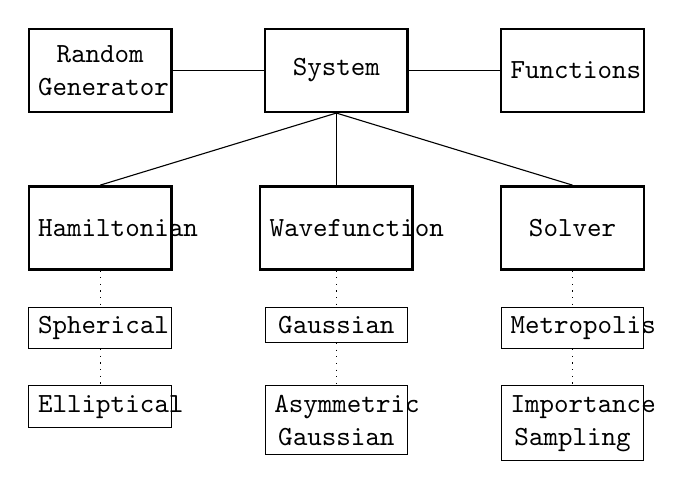
\begin{tikzpicture}
        
        \node (system) [draw, line width=0.3mm, text width=0.13\textwidth, minimum height=30pt, text centered] at (0,2) {\bfseries \texttt{System}};
        
        \node (functions) [draw, line width=0.3mm, text width=0.13\textwidth, minimum height=30pt, text centered] at (3,2) {\bfseries \texttt{Functions} };
        
        \node (random) [draw, line width=0.3mm, text width=0.13\textwidth, minimum height=30pt, text centered] at (-3,2) {\bfseries \texttt{Random \\ Generator} };
        
        \node (wavefunction) [draw, line width=0.3mm, text width=0.14\textwidth, minimum height=30pt, text centered] at (0,0) {\bfseries \texttt{Wavefunction}};
        \node (gauss) [draw, anchor=north, text width=0.13\textwidth, text centered] at (0, -1) {\texttt{Gaussian}};
        \node (asymmgauss) [draw, anchor=north, text width=0.13\textwidth, text centered] at (0, -2) { \texttt{Asymmetric \\ Gaussian}};
        
        \node (solver) [draw, line width=0.3mm, text width=0.13\textwidth, minimum height=30pt, text centered] at (3,0) {\bfseries \texttt{Solver}};
        \node (metropolis) [draw, anchor=north, text width=0.13\textwidth, text centered] at (3, -1) {\texttt{Metropolis}};
        \node (importance) [draw, anchor=north, text width=0.13\textwidth, text centered] at (3, -2) { \texttt{Importance \\ Sampling}};
        
        \node (hamiltonian) [draw, line width=0.3mm, text width=0.13\textwidth, minimum height=30pt, text centered] at (-3,0) {\bfseries \texttt{Hamiltonian}};
        \node (spherical) [draw, anchor=north, text width=0.13\textwidth, text centered] at (-3, -1) {\texttt{Spherical}};
        \node (elliptical) [draw, anchor=north, text width=0.13\textwidth, text centered] at (-3, -2) {\texttt{Elliptical}};
        
        \draw (system.south) -- (wavefunction.north);
        \draw (system.south) -- (hamiltonian.north);
        \draw (system.south) -- (solver.north);
        \draw (system.west) -- (random.east);
        \draw (system.east) -- (functions.west);
        
        \draw [dotted] (hamiltonian.south) -- (spherical.north);
        \draw [dotted] (spherical.south) -- (elliptical.north);
        \draw [dotted] (wavefunction.south) -- (gauss.north);
        \draw [dotted] (gauss.south) -- (asymmgauss.north);
        \draw [dotted] (solver.south) -- (metropolis.north);
        \draw [dotted] (metropolis.south) -- (importance.north);
    \end{tikzpicture}
    \caption{Classes diagram and hierarchy. Elliptical and spherical are Hamiltonian's subclasses, Gaussian and AsymmetricGaussian are Wavefunction's sublclasses, Metropolis and ImportanceSampling are Solver's sublasses.}
    \label{diag:classes_diagram}
\end{figure}

We chose C\texttt{++} as the main programming language to implement the aforementioned methods for this project. This allowed us to keep a good compromise between computational speed and abstraction. As mentioned before, some python algorithms were adopted for post-analysis operations and plots construction. The C\texttt{++} algorithm has been fully object oriented making the code modular, in the sense one can in principle reuse the code for other purposes by only replacing some pieces and keeping the general structure. All the implemented classes can be categorized as follows:
\begin{itemize}
    \item \texttt{System}: contains information on the system as a whole (includes for example the collection of particle) and provides a reference point for communication between the other classes;
    \item \texttt{Solvers}: provide different tools to perform the actual VMC run and evaluate the energy of the system for a chosen Hamiltonian and a selected wavefunction on different complexity levels, depending on the needs;
    \item \texttt{Wavefunctions}: the wavefunction describing the whole system is implemented here, together with the possibility of adjusting the parameters entering in its definition;
    \item \texttt{Hamiltonians}: this includes functions for the evaluation of the local energy;
    \item \texttt{Functions}: this includes some ad-hoc implemented functions that combine elements of the previously cited classes and perform specific tasks requested for the project;
    \item \texttt{RandomGenerator}: it contains functions for the generation of uniform and gaussian distributed random numbers.
\end{itemize}
The code has been documented via Doxygen and the documentation, together with the code itself, can be found at the GitHub link provided at the end of the report, hence hereby we discuss only some of the peculiar points of the implementation. The tests conducted to verify the solidity and the correctness of the results provided by the code will be described in the next section.

For the sake of clarity, the below section of pseudo-code describes the structure that we gave to our implementation. 
\newpage


\begin{minted}[frame=lines, bgcolor=lemonchiffon]{cpp}
#include <defined_classes>

// CREATE OBJECTS
System system(int dimension, int N_particles);

Hamiltonian hamiltonian(&system);
//spherical or elliptical

Wavefunction wavefunction(&systems);
// gaussian or antisymmetric gaussian

Solver solver(&system);
// metropolis or importance

Functions functions(&system);
RandomGenerator randomgenerator(&system);

// set the attributes of the system
system.setHamiltonian(&hamiltonian);
system.setWavefunction(&wavefunction);
system.setSolver(&solver);
system.setRandomGenerator(&randomgenerator);

// perform tasks
functions.task();
\end{minted}



\subsection{SINGLE-PARTICLE WAVEFUNCTION EVALUATION}
According to what previously discussed, for every VMC step we are in need to perform an acceptance test for the proposed move by evaluating a ratio of wavefunctions. Eq.\,\ref{wavefunctions} together with the fact that for each VMC step only one particle is moved, one infers that the acceptance test can be carried out by evaluating only those components in the wavefunction that include information on the moved particle. More in detail, in the non-interacting case if the wavefunction at the step $k$ of the simulation is
\begin{equation*}
    \Psi_T^{k} \equiv \Psi(\bm{R}(t_k)) = \prod_{i=1}^{N} g(\alpha, \bm{r}_i(t_k)) \equiv \prod_{i=1}^N g_i^{(k)}
\end{equation*}
then, if at the step $k+1$ we modify the position of the particle $n$, the wavefunction becomes
\begin{equation*}
    \Psi_T^{k+1} \ = \ g_n^{(k+1)} \, \prod_{\substack{i=1\\ i \neq n}} g_i^{k}
\end{equation*}
Thus the ratio between the wavefunctions appearing in Eq.\,\ref{acceptance_metropolis} and Eq.\,\ref{acceptance_importance} reduces to $\vert g_n^{(k+1)} \vert^2 / \vert g_n^{(k)} \vert^2$, allowing a reduction in the computational time. 


\subsection{RELATIVE POSITION BETWEEN PARTICLES IN THE INTERACTING CASE}
\label{sec:matrix_relative_dist}
The interacting case leads to way more complicated expressions for the wavefunction and the local energy, therefore finding clever way to reduce as much as possible the computational effort is not so trivial as in the non-interacting case. However we noticed the repetitive demand for the same quantities, like the relative positions and relative distances between particles, in different expressions. Hence, we stored those values in proper matrices in order to avoid repetitive re-evaluations of those high time-demanding operations once that the position of the particles is set after a simulation step. The $ij$-th element of the distance matrix $D_{ij}$ is the distance between the particle $i$ and particle $j$: here one can note that this matrix is symmetrical, hence only one half of the off-diagonal values must be computed. In a similar way the $ij$-th element of the relative position matrix $R_{ij} = \bm{r}_i - \bm{r}_j$ is the relative position, in cartesian coordinates, of the particles $i$ with respect to to the particle $j$: this matrix is antisymmetrical, hence, also in this case, only half of the off-diagonal element can be computed. The matrices are built and initialised at the beginning of the program, and after one particle is moved, only the corresponding rows and columns in the matrices are updated.



    
\subsection{CODE PARALLELIZATION}
The code has been parallelized via OpenMP. The strategy we adopted consisted in creating a copy of the system for every thread, each one with the same settings, and the selected number of steps for a single MC run was  equally split into the threads. Each parallel simulation was thus carried with a reduced number of steps and data generated from each thread was saved into different files, successively collected together in a python environment and the analysis was carried on the whole dataset. The  computational time improvement was analyzed on a 4-cores computer, observing a reduction factor in the simulation time which laid between $3.0$ and $3.5$.

A slightly different approach regards the gradient descent process, for which an independent research was launched on every thread, each of them providing us at the end with a different estimate of $\alpha_{GS}$. 




\newpage 

\section{RESULTS}
The analysis of the results produced by our code passed through a series of intermediate and progressive steps, continuously checking the outcomes obtained via the simulation with the analytical formulas, fortunately available for the non-interacting case. We will now proceed with the presentation of the results derived within the context of our project, enlightening the features of any performed simulation and the methods to validate the solidity and efficiency of the code. First we will focus on the runs carried out in non-interacting case both with the brute-force Metropolis algorithm and the importance sampling, proceeding then towards a more detailed statistical analysis through the blocking method. Then the interaction between particles will be introduced, together with the gradient descent method for the research of the $\alpha$ which minimizes the energy and then concluding with the one-body density evaluation.


\subsection{NON-INTERACTING SYMMETRICAL CASE}
\subsubsection{BRUTE-FORCE METROPOLIS ALGORITHM}
At first we chose a spherical potential trap with a simple gaussian trial wavefunction, these obtained by setting $a=0$ and $\beta=1$ into Eq.\,\ref{wavefunctions} and adopting the potential described in Eq.\,\ref{spherical_pot}. In order to obtain a numerical estimation of the ground state energy of the system we first adopted the so called Brute-Force Metropolis algorithm, previously introduced. We performed different simulations varying many parameters of the system and before each of these runs the system was submitted to $10^5$ thermalization steps. This choice has been preserved for each simulation presented from now on in the report. In principle we could have reduced the number of thermalization steps for the most simple configurations, involving for example 1 particle in a 1-dimensional system. However, since the most time-demanding operation is the evaluation of the local energy (not performed for the thermalization steps), the computational time for the initialization is considerably low, even with such an amount of steps and a large number of particles. We notice also that with the highest number of particles adopted for the system ($N=500$), within a $10^5$-steps thermalization process each of them will on average be moved 200 times, which we retained sufficient for the considered Markov chain to converge to the stationary PDF. 

Table \ref{tab:tab_x_metropolis_analytical} reports the results of the analysis of the system's dependence on the number of particles and dimension. The value of $\alpha$ was kept fixed at $\alpha = 0.5$. The corresponding results obtained using the numerical method to evaluate the second derivative are reported in Table \ref{tab:tab_x_metropolis_numerical}. One can immediately notice a reduction in the precision and a significant increase in the simulation time with the numerical approach, hence leaving the only purpose of this second method to perform preliminary tests and qualitative studies. Proceeding, Figure \ref{fig:varying_alpha_noninteract_metropolis}, shows the value of the ground state energy of the system as a function of the parameter $\alpha$ for a particular configuration of the simulation settings, that is $N=10$ particles, 3 dimensions, $2^{21}$ steps and Metropolis step-size $r_{step} = 1.0$. One can immediately notice that the function is convex, which guarantees the existence of one unique minimum point, in accordance to what discussed in the context of the gradient descent method. In this simple case, the convexity of the energy curve as a function of $\alpha$ was expected, as it can be derived from the analytical form available in Eq.\,\ref{energy_analitical}. Some selected results for different $\alpha$ values are reported also in Table \ref{tab:varying_alpha_noninteracting}, referring to simulations performed again for a $3D$ system with $N=10$ particles and $N_{steps}=2^{21}$. This table contains also a comparison between the variance calculated as $\sigma^2_E = (\langle E_L^2 \rangle - \langle E_L \rangle^2)/N_{steps}$ and the variance calculated via the blocking method as explained in Section \ref{sec:blocking_method}.

\afterpage{
\begin{table}[t!]
    \centering
    \begin{tabular}{cccccc}
    \toprule
    $N_{part}$ & $N_{dim}$ & $\langle E_L \rangle$ & $\sigma_E$ & $t_{CPU}\;[s]$ & acc.ratio \\
    \midrule
    1 & 1 & 0.50000 & 0.00000 & 0.250 & 0.7293 \\
    1 & 2 & 1.0000 & 0.00000 & 0.277 & 0.5958 \\
    1 & 3 & 1.5000 & 0.00000 & 0.293 & 0.5053 \\
    \midrule
    10 & 1 & 5.0000 & 0.00000 & 0.397 & 0.7290 \\
    10 & 2 & 10.000 & 0.00000 & 0.426 & 0.5956 \\
    10 & 3 & 15.000 & 0.00000 & 0.453 & 0.5047 \\
    \midrule
    100 & 1 & 50.000 & 0.00000 & 1.967 & 0.7287 \\
    100 & 2 & 100.00 & 0.00000 & 2.084 & 0.5950 \\
    100 & 3 & 150.00 & 0.00000 & 2.388 & 0.5043 \\
    \midrule
    500 & 1 & 250.00 & 0.00000 & 20.695 & 0.7293 \\
    500 & 2 & 500.00 & 0.00000 & 22.008 & 0.5961 \\
    500 & 3 & 750.00 & 0.00000 & 21.776 & 0.5051 \\
    \bottomrule
    \end{tabular}
    \caption{The table reports the results of the simulations performed in the non-interacting case using a simple gaussian trial wavefunction and a brute-force Metropolis sampling method with $N_{therm}=10^5$, $N_{steps}=2^{21}$, step-size set to $r_{step}=1.0$ and constant value for $\alpha=0.5$. The local energy is evaluated exploiting the analytical formula and $\sigma_E$ is the error on $\langle E_L \rangle$ estimated from the standard deviation of of the $E_L$ samples generated during the run. }
    \label{tab:tab_x_metropolis_analytical}
\end{table}

\begin{table}[h!]
    \centering
    \begin{tabular}{cccccc}
    \toprule
    $N_{part}$ & $N_{dim}$ & $\langle E_L \rangle $ & $\sigma_E$ & $t_{CPU}$ & acc.ratio \\
    \midrule
    1 & 1 & 0.5000000000 & 7\e-10 & 0.497 & 0.7290 \\
    1 & 2 & 1.000000000 & 1\e-9 & 0.631 & 0.5949 \\
    1 & 3 & 1.500000000 & 2\e-9 & 0.799 & 0.5050 \\
    \midrule
    10 & 1 & 5.000000006 & 2\e-9 & 2.217 & 0.7296 \\
    10 & 2 & 10.000000000 & 3\e-9 & 2.975 & 0.5960 \\
    10 & 3 & 15.000000010 & 5\e-9 & 4.035 & 0.5051 \\
    \midrule
    100 & 1 & 49.999999913 & 7\e-9 & 20.71 & 0.7287 \\
    100 & 2 & 99.99999991 & 1\e-8 & 28.49 & 0.5957\\
    100 & 3 & 149.99999965 & 2\e-8 & 37.02 & 0.5057 \\
    \midrule
    500 & 1 & 250.99999950 & 1\e-8 & 237.05 & 0.7298 \\
    500 & 2 & 500.00000067 & 2\e-8 & 347.24 & 0.5952 \\
    500 & 3 & 749.99999921 & 3\e-8 & 413.98 & 0.5045 \\
    \bottomrule
    \end{tabular}
    \caption{The table reports the results of the simulations in the non-interacting case using a simple gaussian trial wavefunction and a brute-force Metropolis sampling method with $N_{therm}=10^5$,  $N_{steps}=2^{21}$, step-size set to $r_{step}=1.0$ and constant value for $\alpha=0.5$. The local energy is evaluated exploiting the numerical second derivative and $\sigma_E$ is the error on $\langle E_L \rangle$ estimated from the standard deviation of the $E_L$ samples generated during the run. }
    \label{tab:tab_x_metropolis_numerical}
\end{table}
}



\subsubsection{IMPORTANCE SAMPLING}
The immediate improvement of this simple model was the inclusion of the importance sampling. This allowed us to bias the random walk in the configuration space according to the probability distribution, leading thus to a higher number of accepted steps in the Monte Carlo run. As for the Brute Force Metropolis, results for fixed $\alpha=0.5$ obtained with the analytical and numerical evaluation of the local energy are reported respectively in Table \ref{tab:tab_x_importance_analytical} and Table \ref{tab:tab_x_importance_numerical}. The estimated energy as a function of $\alpha$ for a $3D$ system populated by 10 particles is reported in Figure \ref{fig:varying_alpha_noninteract_importance} with some selected results in Table \ref{tab:varying_alpha_noninteracting}. All the simulations cited above have been carried out with $2^{21}$ Monte Carlo steps and $\delta t = 0.1$. 


\afterpage{
\begin{table}[t!]
    \centering
    \begin{tabular}{cccccc}
    \toprule
    $N_{part}$ & $N_{dim}$ & $\langle E_L \rangle$ & $\sigma_E$ & $t_{CPU}$ & acc. ratio \\
    \midrule
    1 & 1 & 0.50000 & 0.00000 & 0.373 & 0.9928  \\
    1 & 2 & 1.0000 & 0.00000 & 0.385 & 0.98877 \\
    1 & 3 & 1.5000 & 0.00000 & 0.432 & 0.9857 \\
    \midrule
    10 & 1 & 5.0000 & 0.00000 & 0.714 & 0.9929 \\
    10 & 2 & 10.000 & 0.00000 & 0.792 & 0.9889 \\
    10 & 3 & 15.000 & 0.00000 & 0.793 &  0.9858 \\
    \midrule
    100 & 1 & 50.000 & 0.00000 & 4.197 & 0.9929 \\
    100 & 2 & 100.00 & 0.00000 & 4.378 & 0.9887 \\
    100 & 3 & 150.00 & 0.00000 &  4.339 & 0.9856 \\
    \midrule
    500 & 1 & 250.00 & 0.00000 & 36.624 & 0.9929 \\
    500 & 2 & 500.00 & 0.00000 & 39.380 & 0.9888 \\
    500 & 3 & 750.00 & 0.00000 & 39.965 & 0.9858 \\
    \bottomrule
    \end{tabular}
    \caption{The table reports the results of the simulations in the non-interacting case using a simple gaussian trial wavefunction and the importance sampling method with $N_{therm}=10^5$, $N_{steps}=2^{21}$, $\delta t = 0.1$ and constant value for $\alpha=0.5$. The local energy is evaluated exploiting the analytical formula and $\sigma_E$ is the error on $\langle E_L \rangle$ estimated from the standard deviation of the $E_L$ samples generated during the run. }
    \label{tab:tab_x_importance_analytical}
\end{table}

\begin{table}[h!]
    \centering
    \begin{tabular}{cccccc}
    \toprule
    $N_{part}$ & $N_{dim}$ & $\langle E_L \rangle$ & $\sigma_E$ & $t_{CPU}$ & acc.ratio \\
    \midrule
    1 & 1 & 0.5000000027 & 7\e-10 & 0.761 & 0.9928 \\
    1 & 2 & 1.000000000 & 1\e-9 & 0.961 & 0.9888 \\
    1 & 3 & 1.500000004 & 2\e-9 &  1.332 & 0.9856\\
    \midrule
    10 & 1 & 4.999999937 & 2\e-9 & 3.311 & 0.9928 \\
    10 & 2 & 10.000000039 & 3\e-9 & 5.772 & 0.9887 \\
    10 & 3 & 15.000000053 & 5\e-9 & 8.097 & 0.9857 \\
    \midrule
    100 & 1 & 49.999999990 & 7\e-9 & 31.444 & 0.9929 \\
    100 & 2 & 99.99999966 & 1\e-8 & 55.850 & 0.9888 \\
    100 & 3 & 150.00000048 & 2\e-8 & 85.201 & 0.9857 \\
    \midrule
    500 & 1 & 250.00000078 & 1\e-8 & 323.70 & 0.9927 \\
    500 & 2 & 500.00000208 & 2\e-8 & 540.58 & 0.9886 \\
    500 & 3 & 749.99999858 & 3\e-8 & 877.82 & 0.9859 \\
    \bottomrule
    \end{tabular}
    \caption{The table reports the results of the simulations in the non-interacting case using a simple gaussian trial wavefunction and the importance sampling method with $N_{therm}=10^5$, $N_{steps}=2^{21}$, $\delta t = 0.1$ and a constant value of $\alpha=0.5$. The local energy is calculated exploiting the numerical evaluation of the second derivative and $\sigma_E$ is the error on $\langle E_L \rangle$ estimated from the standard deviation of the $E_L$ samples generated during the run.  }
    \label{tab:tab_x_importance_numerical}
\end{table}
}

Even if simple and primitive, this model allowed us to test many of the fundamental parts of the code and made us understand how to fine-tune some parameters involved in the problem. For example, we analysed the effects of the time-step length $\delta t$ in the importance sampling case, concluding that a good choice for the parameter could be $\delta t = 0.1$. Our choice is justified by the fact that this value of $\delta t$ provides us both with a relatively high speed in the exploration of the space of configurations and a high acceptance ratio. In fact, it make large steps more likely to be proposed for the particles (according to Eq.\,\ref{new_position_importance}), still having number of accepted moves close to the actual number of performed steps. Both these aspects can be appreciated in Figure \ref{fig:dt_importance_sampling} and Figure \ref{fig:correlation_varying_dt}: the former shows the acceptance ratio as a function of $\delta t$, the latter demonstrates that a smaller value for the time-step introduces more correlation between data. For the realization of this second graph the parameter $\alpha$ was set to 0.4 in order to introduce some statistical fluctuations in the data, otherwise absent in the case of $\alpha=0.5$.

\afterpage{
\begin{table}[t!]
    \centering
    \begin{tabular}{ccccc}
    \toprule
        \multicolumn{5}{c}{Metropolis} \\
        \midrule
        $\alpha$ & $\langle E_L \rangle$ & $\sigma_E$ & $\sigma_B$ & acc.ratio \\
         \midrule
        $0.3$ & 17.000 & 0.001 & 0.02 & 0.60313 \\
        $0.4$ & 15.3768 & 0.0006 & 0.007 & 0.54918 \\
        $0.5$ & 15.0000 & 0.0000 & 0.0000 & 0.50533 \\
        $0.6$ & 15.2492 & 0.0005 & 0.006 & 0.46724\\
        $0.7$ & 15.8461 & 0.0009 & 0.01 & 0.43341\\
        \midrule
        \midrule
         \multicolumn{5}{c}{Importance Sampling} \\
        \midrule
        $\alpha$ & $\langle E_L \rangle$ & $\sigma_E$ & $\sigma_B$ & acc.ratio \\
        \midrule
        $0.3$ & 16.9924 & 0.001 & 0.02 & 0.99343\\
        $0.4$ & 15.3826  & 0.0006 & 0.007 & 0.98982\\
        $0.5$ & 15.0000 & 0.0000 & 0.0000 & 0.98587 \\
        $0.6$ & 15.2471 & 0.0005 & 0.005 & 0.98123\\
        $0.7$ & 15.8468 & 0.0009 & 0.008 & 0.97630\\
        \bottomrule
    \end{tabular}
    \caption{Results of the simulations for different values of the variational parameter $\alpha$. Here $\sigma_E$ is the error on $\langle E_L \rangle$ estimated from the standard deviation of the $E_L$ samples generated during the run, while $\sigma_B$ comes from the blocking analysis. For both the brute-force Metropolis case and the importance sampling case we used 10 particles in 3 dimensions, $N_{therm}=10^5$ and $N_{steps}=2^{21}$. The chosen step-size for the Metropolis algorithm was $r_{step}=1.0$ and the time step-size for the Importance Sampling was $\delta t = 0.1$. }
    \label{tab:varying_alpha_noninteracting}
\end{table}
}

\afterpage{
\begin{figure}[h!]
    \centering
    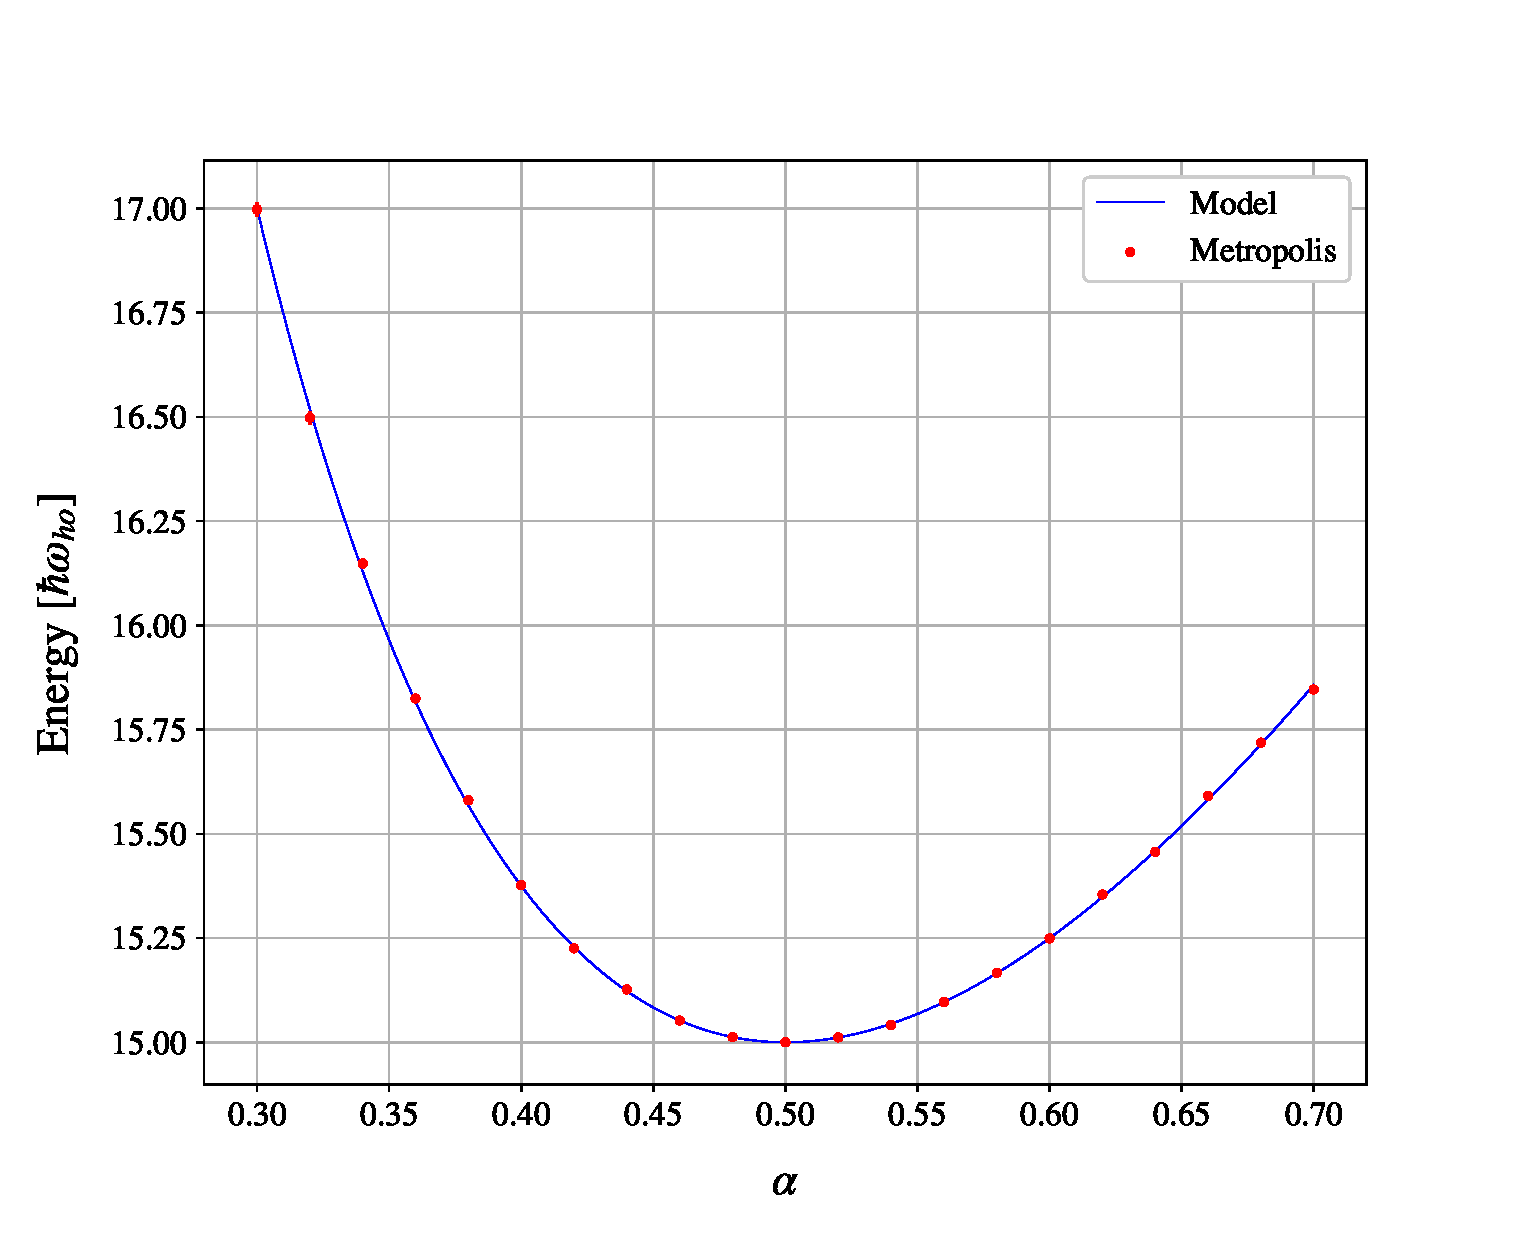
\includegraphics[scale=0.37]{images/varying_alpha_noninteract_metropolis.eps}
    \caption{The figure reports the energy estimates as a function of $\alpha$ generated by various VMC simulations exploiting the brute-force Metropolis algorithm with $N_{therm}=10^5$, $N_{steps}=2^{21}$ and $r_{step}=1.0$. The curve is referred to a $3D$ system with $N=10$ non-interacting particles. For some of the points the errorbar is too small to be seen. }
    \label{fig:varying_alpha_noninteract_metropolis}
\end{figure}
}

\afterpage{
\begin{figure}[h!]
    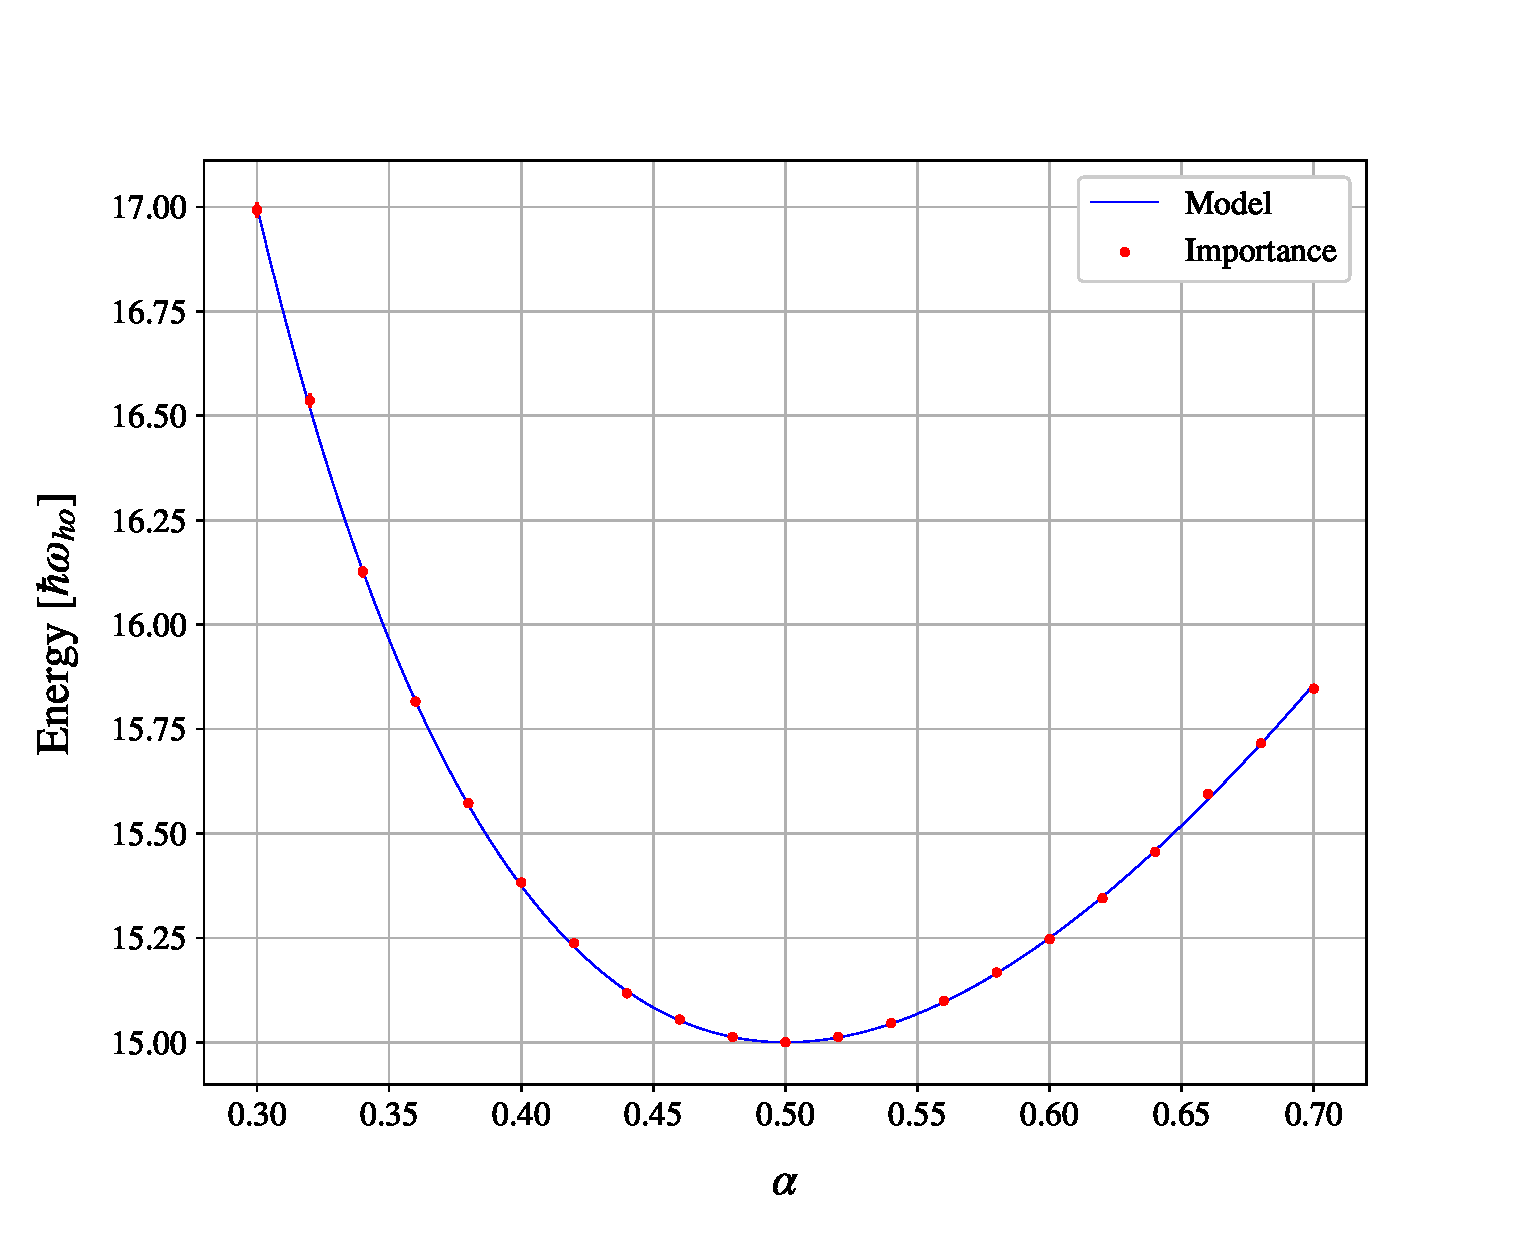
\includegraphics[scale=0.37]{images/varying_alpha_noninteract_importance.eps}
    \caption{The figure reports the energy estimates as a function of $\alpha$ generated by various VMC simulations exploiting the importance sampling with $N_{therm}=10^5$, $N_{steps}=2^{21}$, $\delta t = 0.1$. The curve is referred to a $3D$ system with $N=10$ non-interacting particles. For some of the points the errorbar is too small to be seen. }
    \label{fig:varying_alpha_noninteract_importance}
\end{figure}
}

\afterpage{
\begin{figure}[h!]
    \centering
    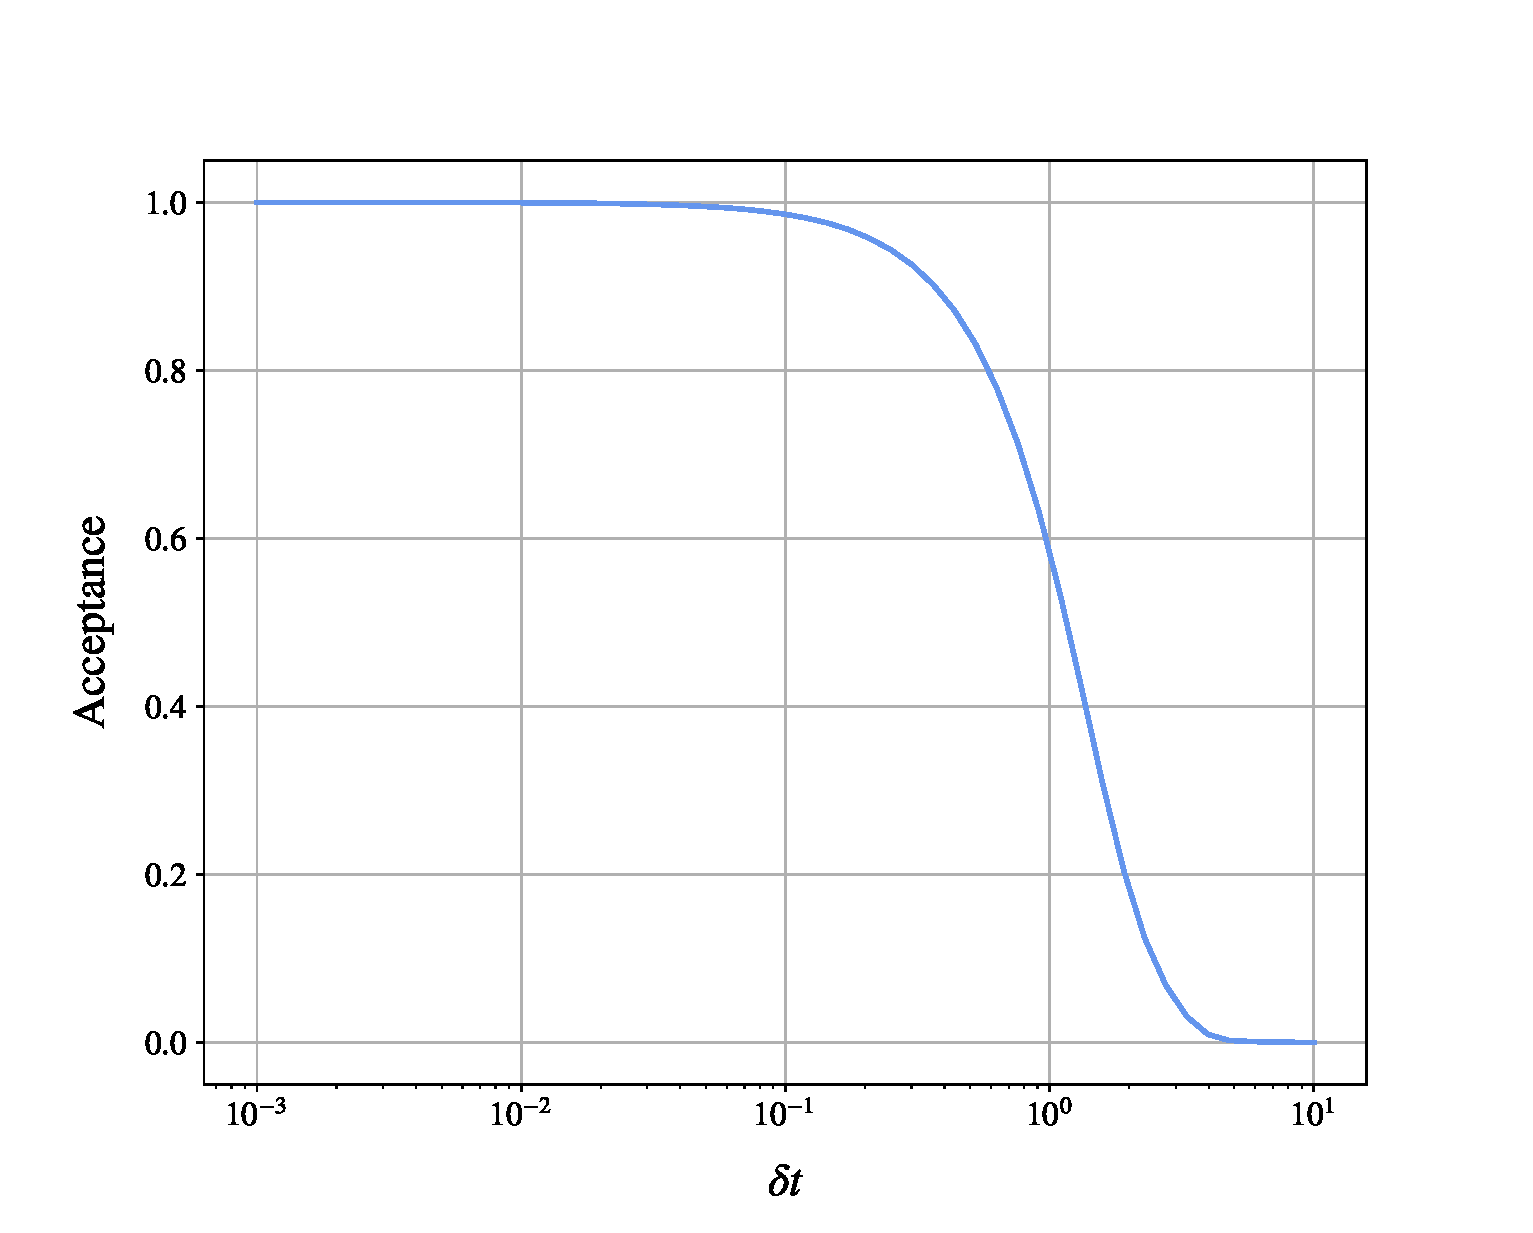
\includegraphics[scale=0.37]{images/varying_dt.eps}
    \caption{Acceptance ratio as a function of the time-step $\delta t$ in the context of VMC simulation performed with the importance sampling technique. Each run is conducted with $N_{therm}=10^5$, $N_{steps}=2^{21}$ and involves a system of $10$ non-interacting particles in 3-dimensions with $\alpha=0.5$.}
    \label{fig:dt_importance_sampling}
\end{figure}

\begin{figure}[h!]
    \centering
    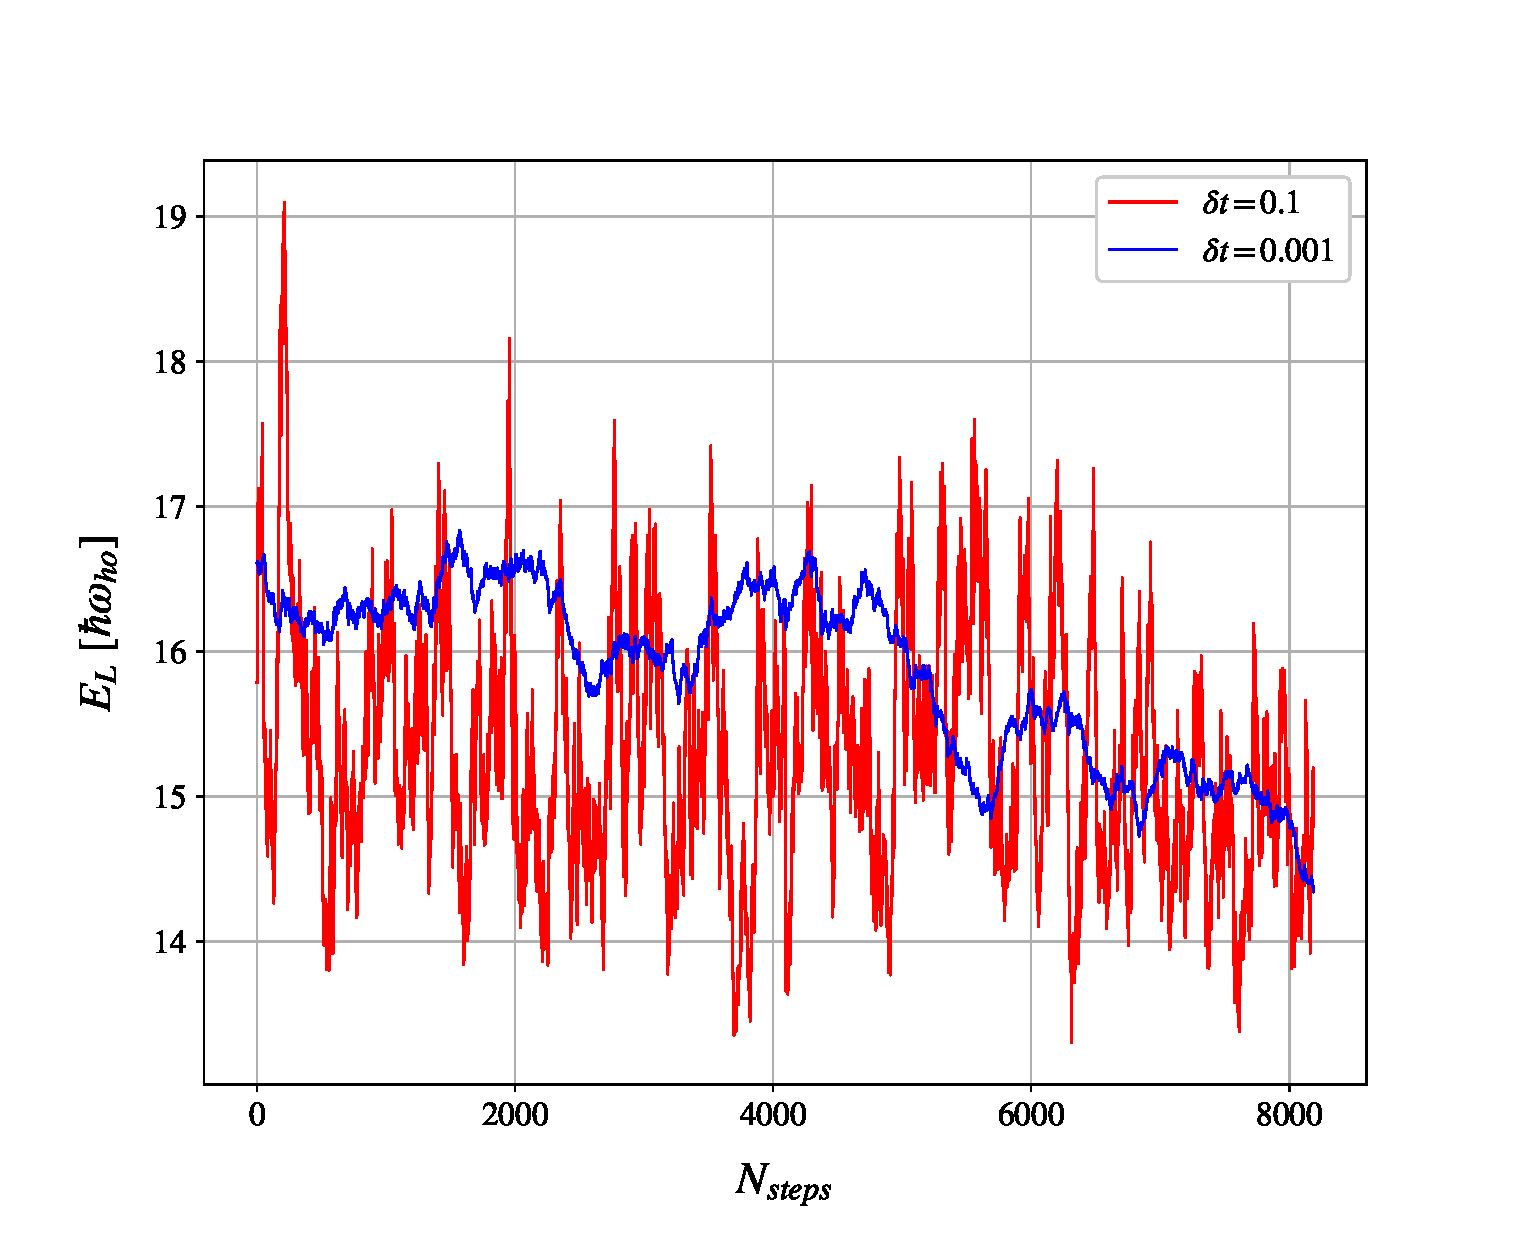
\includegraphics[scale=0.37]{images/correlation_different_deltat.eps}
    \caption{Local energy evaluated in each step of a VMC simulation after $N_{therm}=10^5$. A $3D$ system populated by 10 non-interacting particles inserted in a spherical potential is considered here. The image shows two curves for the chosen parameter $\delta t=0.001$ and $\delta t = 0.1$ used for the importance sampling method. The variational parameter $\alpha$ is set as constant to 0.4 to introduce some statistical fluctuations in the data, absent for $\alpha=0.5$. }
    \label{fig:correlation_varying_dt}
\end{figure}
}

\subsubsection{STATISTICAL ANALYSIS THROUGH BLOCKING METHOD}
\textcolor{white}{ciao\\}
As previously stated, Table \ref{tab:varying_alpha_noninteracting} contains estimations of the error affecting $\langle E_L(\alpha) \rangle$ obtained directly from the variance provided by the VMC simulations and the one obtained with the blocking technique. The python script that provided us with these latter results is based on the theoretical background described in Section \ref{sec:blocking_method}. The consistency of the mentioned script was also tested, in particular for what concerns the convergence of the estimate for  $\sigma_\mu^2$ (see Eq.\,\ref{eq:blocking_method}) to a finite value after a sufficiently high number of blocking iterations. In Figure \ref{fig:blocking_analysis} we present the values of $\sigma_k$ after each iteration of the mentioned method: the results are derived from a simulation performed with $2^{23}$ steps on a $3D$ system containing $N=10$ non-interacting particles inserted in a spherical potential. The sampling was performed through the Metropolis-Hastings algorithm using $\delta t=0.1$ and the variational parameter was again set to $\alpha=0.4$. As expected, we can observe that $\sigma_k$ reaches a plateau for sufficiently high values of $k$, and then an erratic behaviour enters into play, this due to the progressive reduction of the amount of points on which the variance is estimated. 

\afterpage{
\begin{figure}[h!]
    \centering
    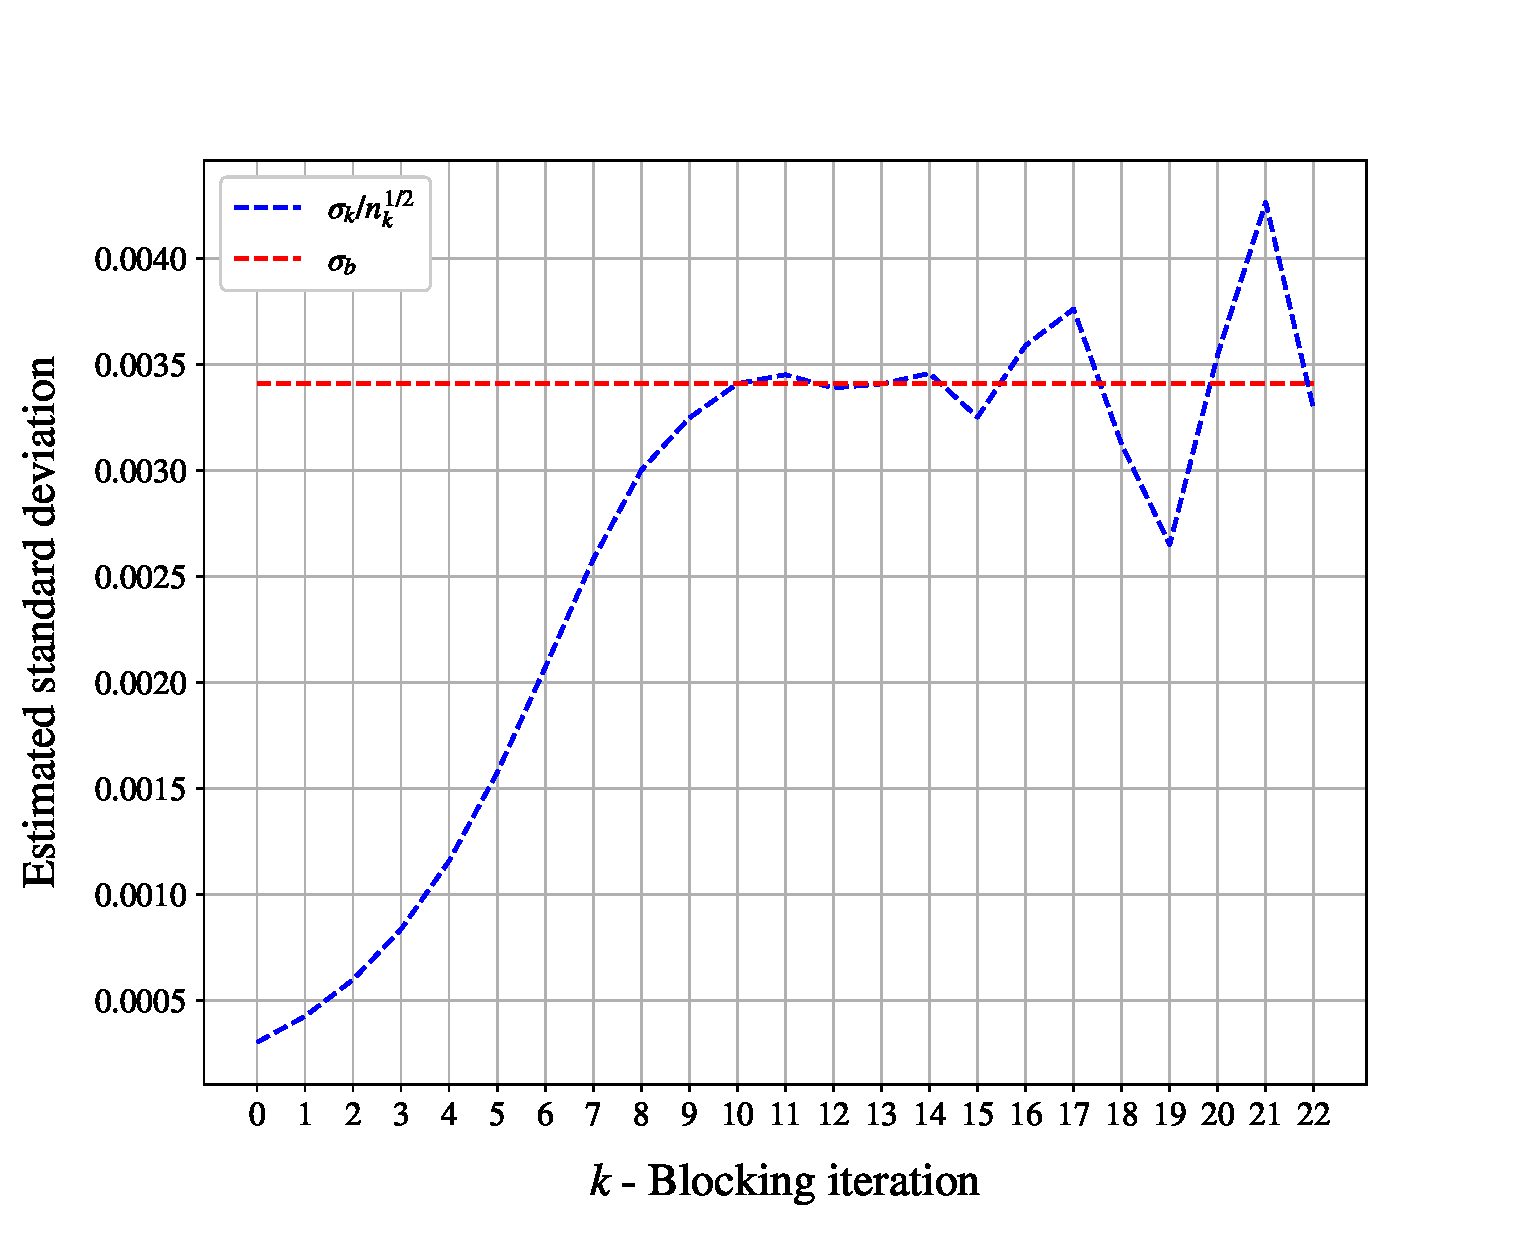
\includegraphics[scale=0.37]{images/sigma_blocking_behaviour.eps}
    \caption{The figure shows the behaviour of the variance estimation provided by the blocking technique implemented in a python script. The simulation was performed with $N_{therm}=10^5$ and $N_{steps}=2^{23}$ on a non-interacting $3D$ system characterized by $\alpha=0.4$ and populated by 10 particles. The Metropolis-Hastings algorithm with $\delta t =0.1$ was adopted for the sampling. }
    \label{fig:blocking_analysis}
\end{figure}}


\subsection{INTERACTING CASE}
Subsequently we moved on to the interacting and asymmetrical case with trial wavefunction given by Eq.\,\ref{wavefunctions} and Hamiltonian described in Eq.\,\ref{hamiltonian} and Eq.\,\ref{elliptical_pot}. At first we compared results with those obtained from the symmetrical case, again to test the solidity of our code: this could be done by setting $\beta=1$, $w_z = w_{ho} = 1$ and the s-wave scattering length $a$ to 0. We verified that the results were coincident with those obtained in the non-interacting case, using both the Brute-force Metropolis algorithm and the importance sampling (see Appendix \ref{appendix:interacting_reduced_as_non_interacting}). From now on we will omit to specify the sampling algorithm used for each simulation, since all the next results were derived exploiting the Metripolis-Hastings one: this choice was driven by the fact that the this technique provides the combination of a higher acceptance ratio and better statistical sampling of the data. Furthermore, the variance on the energy value provided by each VMC was estimated through the blocking analysis. From now on, this information will be omitted too. \\

After the aforementioned consistency check we set the parameters' values $\omega_z = \beta = 2.82843$ and $a = 0.0043$ and ran the simulations for $N=10,50,100$ particles while varying $\alpha$. The simulations for 10 and 50 particles were carried out using $2^{21}$ steps, while in the case of 100 particles the high computational time imposed us a reduction of the number of steps to $2^{19}$. The parameter $\delta t = 0.1$ was the same for every run and the corresponding results are reported in Table \ref{tab:varying_alpha_interacting}. Furthermore, as an example the results obtained for 10 particles are reported in Figure \ref{fig:asymm_symm_comparison}, compared with their homologous obtained in the non-interacting symmetrical case. Figure \ref{fig:E_over_N} reports a comparison between the energy per particle as a function of the variational parameter $\alpha$ obtained for the three different values of $N$. \\


\afterpage{
\begin{table}[t!]
    \centering
    \begin{tabular}{cccc}
    \toprule
        \multicolumn{4}{c}{$N=10$} \\
        \midrule
        $\alpha$ & $\langle E_L \rangle$ & $\sigma_B$ & acc.ratio \\
        \midrule
        $0.3$ & 27.59 & 0.02 & 0.98185 \\
        $0.4$ & 24.969 & 0.008 & 0.97230 \\
        $0.5$ & 24.3991 & 0.0003 & 0.96178  \\
        $0.6$ & 24.822 & 0.006 & 0.94964 \\
        $0.7$ & 25.83 & 0.01 & 0.93758 \\
        \midrule
        \midrule
        \multicolumn{4}{c}{$N=50$} \\
        \midrule
        $\alpha$ & $\langle E_L \rangle$ & $\sigma_B$ & acc. ratio \\
        \midrule
        $0.3$ & 142.8 & 0.1 & 0.97840 \\
        $0.4$ & 129.81 & 0.04 & 0.96866 \\
        $0.5$ & 127.287 & 0.006 & 0.95759 \\
        $0.6$ & 129.90 & 0.03 & 0.94583 \\
        $0.7$ & 135.54 & 0.06 & 0.93361 \\
        \midrule
        \midrule
        \multicolumn{4}{c}{$N=100$} \\
        \midrule
        $\alpha$ & $\langle E_L \rangle$ & $\sigma_B$ & acc. ratio \\
        \midrule
        $0.3$ & 296.8 & 0.4 & 0.97610 \\
        $0.4$ & 271.2 & 0.1 & 0.96336 \\
        $0.5$ & 266.51 & 0.07 &  0.93323\\
        $0.6$ & 272.8 & 0.2 &   0.94392\\
        $0.7$ & 285.1 & 0.2 &  0.92906\\
        \bottomrule
    \end{tabular}
    \caption{The table reports the results of the simulations for different values of the variational parameter $\alpha$ for a $3D$ system constituted by $N=10,\;50,\;100$ particles. The simulations were performed exploiting the Metropolis-Hastings algorithm with $\delta t=0.1$, $N_{therm}=10^5$ and $N_{steps}=2^{21}$ for $N=10,\;50$, while and $N_{steps}=2^{19}$ for $N=100$. }
    \label{tab:varying_alpha_interacting}
\end{table}

\begin{figure}[h!]
    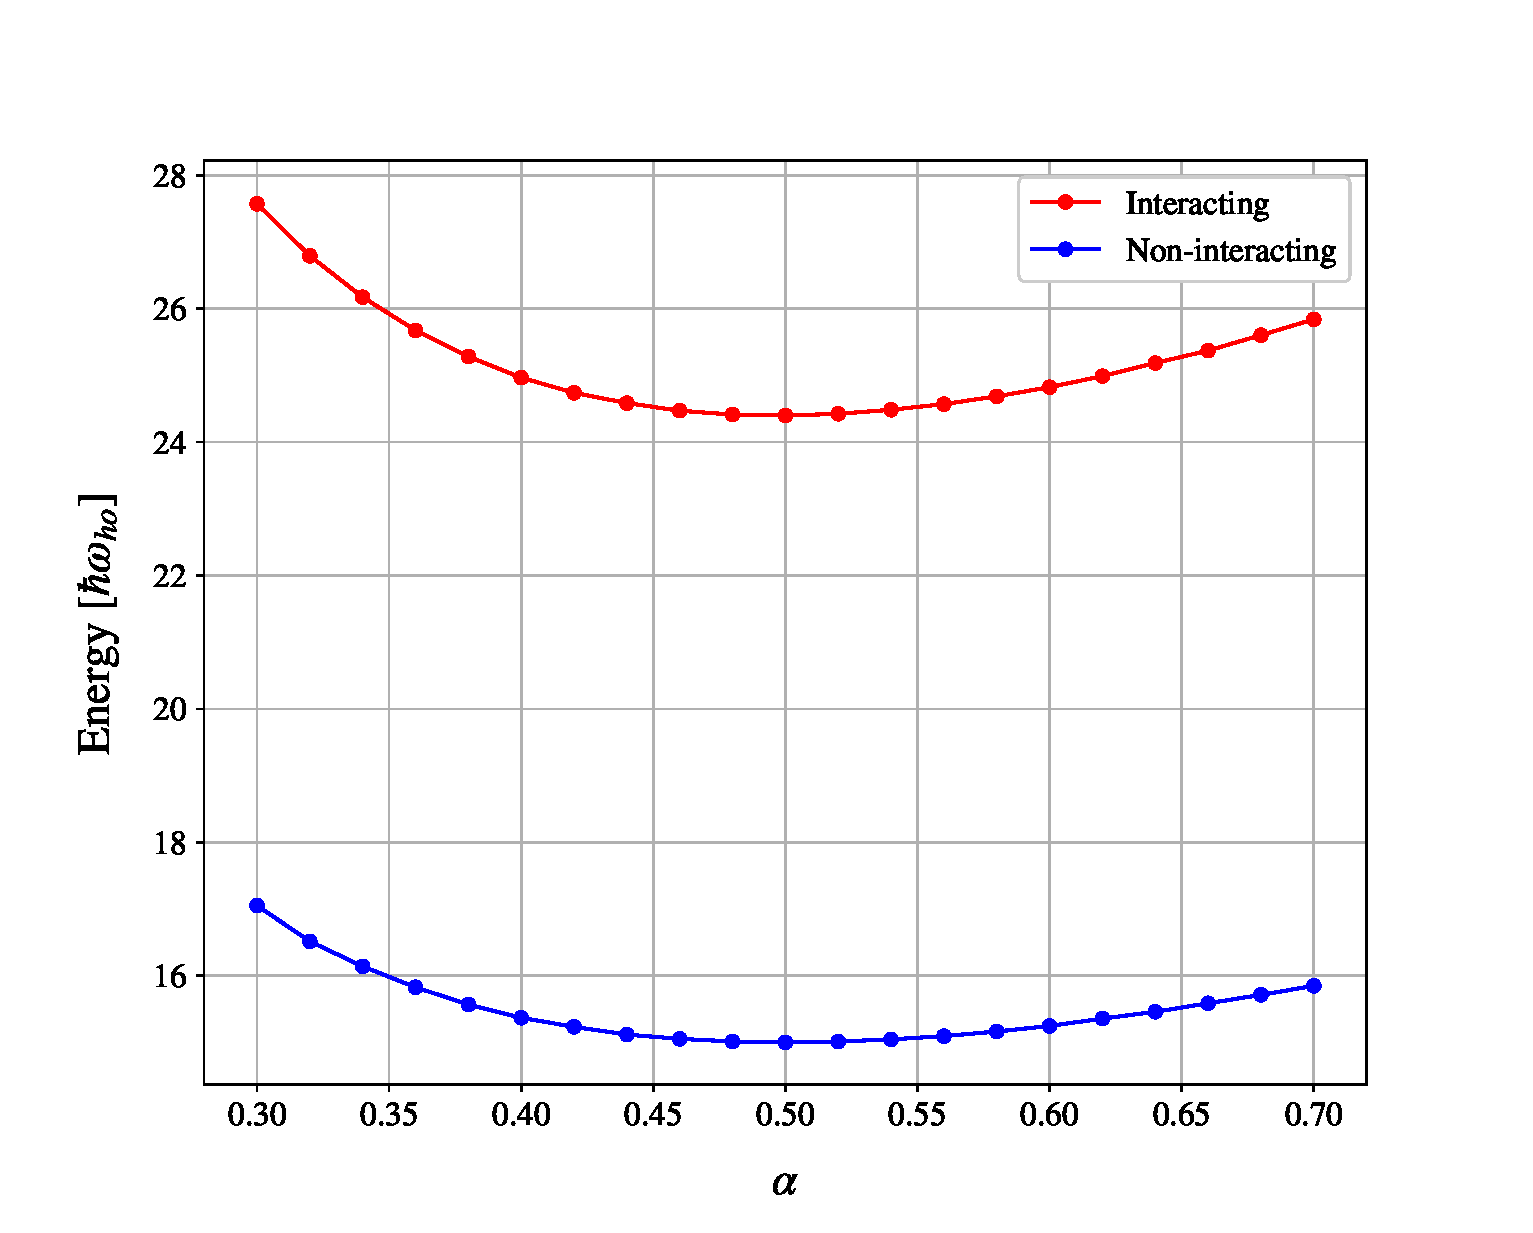
\includegraphics[scale=0.37]{images/varying_alpha_comparison_interacting_and_not.eps}
    \caption{The figure reports the energy estimates as a function of $\alpha$ generated by various VMC simulations exploiting the importance sampling algorithm with $N_{therm}=10^5$, $N_{steps}=2^{21}$, $\delta t = 0.1$. The curves are referred to a $3D$ system populated respectively by 10 non-interacting particles in a spherical potential and 10 interacting particles in an elliptical potential. The errorbars are too small to be seen. }
    \label{fig:asymm_symm_comparison}
\end{figure}
}

\afterpage{
\begin{figure}[t!]
    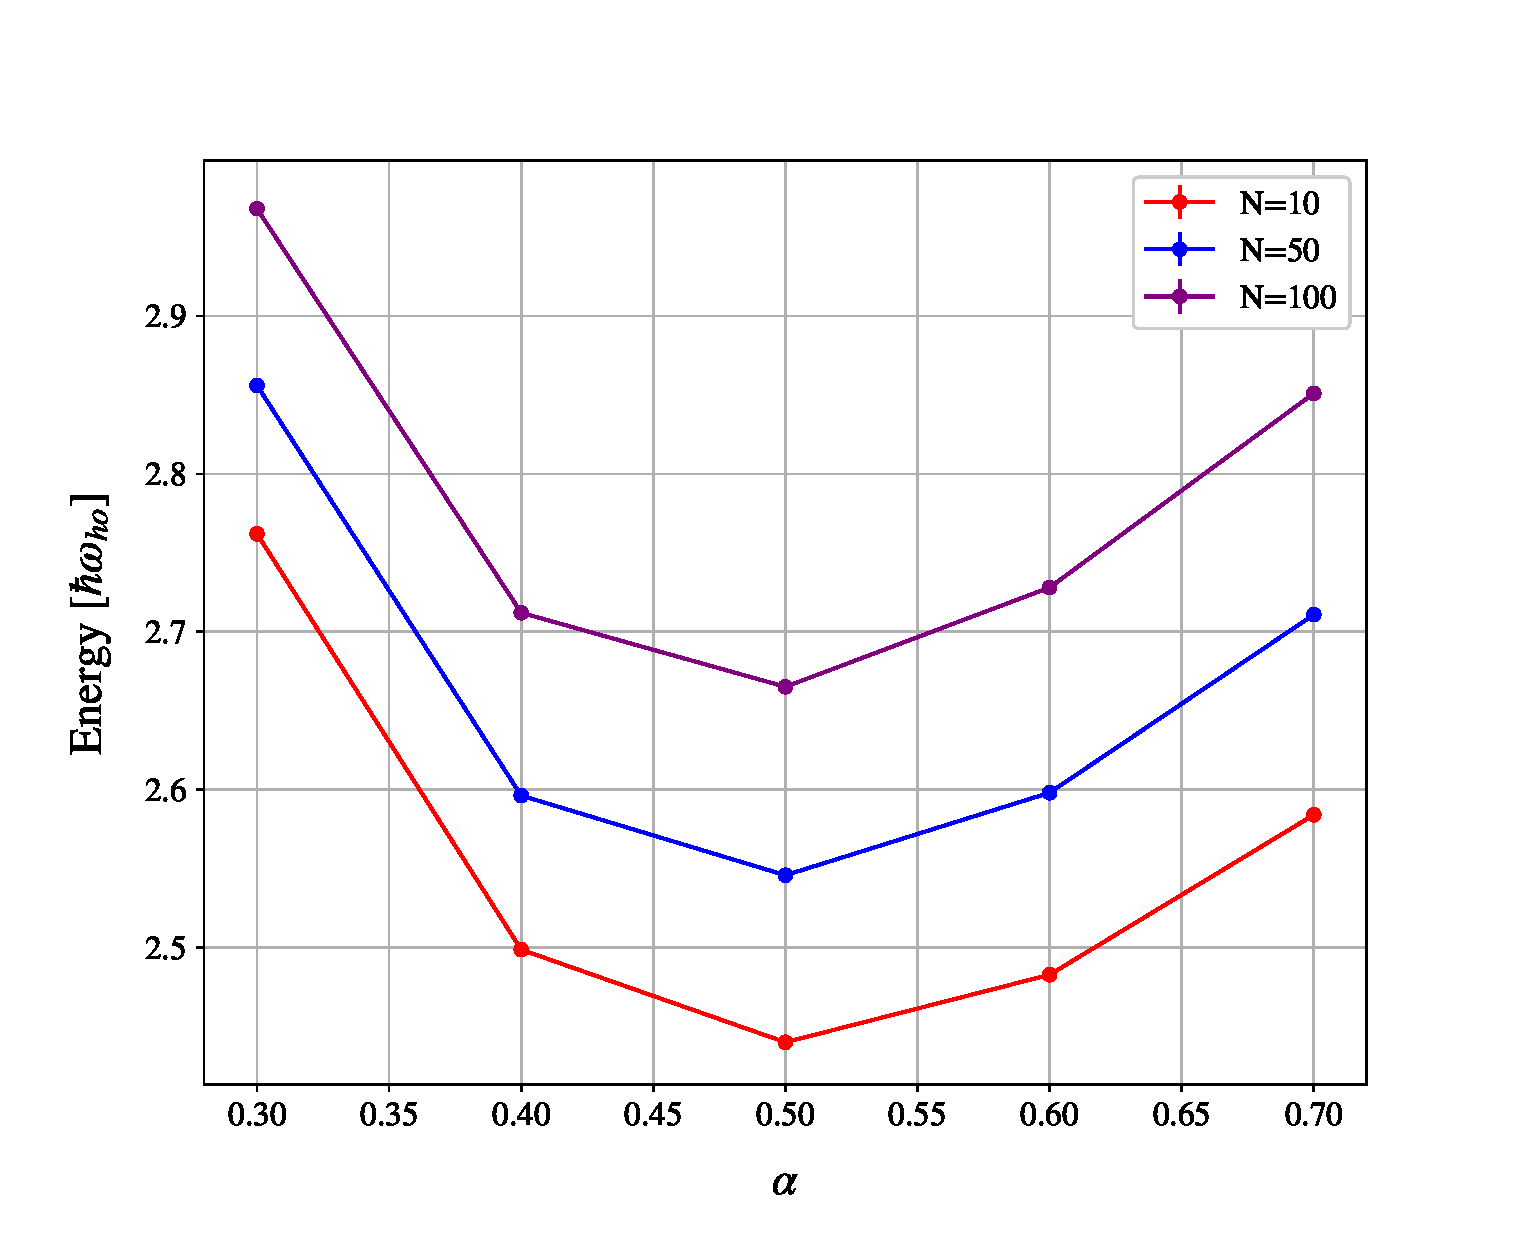
\includegraphics[scale=0.37]{images/energy_over_N.eps}
    \caption{The figure reports the average energy per particle as a function of $\alpha$ generated by various VMC simulations exploiting the importance sampling algorithm with $N_{therm}=10^5$ and $\delta t = 0.1$. The curves are referred to a $3D$ system populated respectively by 10, 50 and 100 interacting particles in an elliptical potential. The number of employed steps was $2^{21}$ for $N=10$ and $N=50$, while $2^{19}$ for $N=100$. }
    \label{fig:E_over_N}
\end{figure}}


\subsection{GRADIENT DESCENT}
\label{sec:gradient_descent_results}
When considering the interaction between particles, a possible proof of the convexity of the function describing $\langle E_L \rangle$ as a function of $\alpha$ is non-trivial, thus in principle we can not state with absolute confidence that the curve is convex. However, as we can see from the latest figures, the behaviour of $\langle E_L \rangle$ as a function of $\alpha$ still encourages us to exploit the gradient descent method to research for  $\alpha_{GS}$ which minimizes the energy of the system. Before proceeding with the actual investigation in the interacting case, we tested the correct functioning of our code by applying it to a non-interacting system. In this simple case, it is well known that the optimal value of the variational parameter is $\alpha_{GS}=0.5$ and this result is independent of the number of particles and dimensionality. Therefore we expect to reach a convergence to this value whatever the adopted configuration. In particular, when considering particles without interaction we have at our disposal the analytical expression for the total energy of the system (see Eq.\,\ref{energy_analitical}) and the convexity of it is easy to prove. This ensures us that, if the method is capable in reaching a convergence for a sufficiently small value of the so-called learning rate $\gamma$ appearing in Eq.\,\ref{alpha_k}, the gradient descent will lead to a proper estimation of $\alpha_{GS}$. Table \ref{tab:gradient_descent_noninteracting} reports the results obtained with the application of the gradient descent method to a 3-dimensional system of 1, 10 and 100 non-interacting particles. Each VMC run was performed with $\delta t=0.1$ and $10^5$ thermalization steps, followed by another $10^5$ for the actual evaluation of the quantities reported in Eq.\,\ref{dEnergy_dalpha}. The learning rate was properly chosen for each configuration and the tolerance on the derivative was fixed to $\varepsilon=10^{-8}$ with no limit on the maximum number of iterations. The stability of the algorithm was also tested by performing the descent starting from two different guesses for the variational parameter, namely $\alpha_0=0.4$ and $\alpha_0=0.6$.

\afterpage{
\begin{table}[t!]
    \centering
    \begin{tabular}{ccccc}
    \toprule
        $N$ & $\gamma$ & $\alpha_0$ & $\alpha_{best}$ & $N_{conv}$ \\
        \midrule
        1 & 1\e-2 & 0.4 & 0.500 & 285 \\
        1 & 1\e-2 & 0.6 & 0.500 & 295 \\
        10 & 1\e-2 & 0.4 & 0.500 & 21 \\
        10 & 1\e-2 & 0.6 & 0.500 & 23 \\
        100 & 1\e-3 & 0.4 & 0.500 & 24 \\
        100 & 1\e-3 & 0.6 & 0.500 & 26 \\
        \bottomrule
    \end{tabular}
    \caption{Convergence analysis for the energy minimization process performed on a $3D$ non-interacting system of 1, 10, 100 particles in a spherical potential. The simulations were performed with $10^5$ steps for both thermalization and actual run, adopting the importance sampling with $\delta t = 0.1$, adjustable $\gamma$ and tolerance $\varepsilon=10^{-8}$. $N_{conv}$ refers to the number of gradient descent steps to get to convergence and $\alpha_0$ is the initial guess selected for the variational parameter.}
    \label{tab:gradient_descent_noninteracting}
\end{table}


\begin{table}[h!]
    \centering
    \begin{tabular}{cccccc}
        \toprule
        $N$ & $\alpha_{0}$ & $\alpha_{best}$ & $\gamma_{min}$ & $N_{steps-max}$ & $N_{conv}$ \\
        \midrule
        10 & 0.4 & 0.49751 & 1\e-3 & 1\e5 & 74 \\
        10 & 0.6 & 0.49751 & 1\e-3 & 1\e5 & 74 \\
        50 & 0.4 & 0.48881 & 1\e-5 & 2\e5 & 21 \\
        50 & 0.6 & 0.48939 & 1\e-5 & 2\e5 & 21 \\
        100 & 0.4 & 0.481 & 1\e-5 & 5\e5 & 16 \\
        100 & 0.6 & 0.483 & 1\e-5 & 5\e5 & 11 \\
        \bottomrule
    \end{tabular}
    \caption{Convergence analysis for the energy minimization process performed on a interacting system of 10, 50 and 100 particles in a elliptical potential. A detailed description of the algorithm implemented for reaching these results is described in Paragraph \ref{sec:gradient_descent_results}. Here $\gamma_{min}$ and $N_{steps-max}$ are the minimum learning rate and maximum number of VMC steps used to perform a single run, while $N_{conv}$ is the iteration number at which the algorithm was stopped. Each run was performed employing the importance sampling with $\delta t = 0.1$ and $N_{therm}=10^5$. }
    \label{tab:gradient_descent_interacting}
\end{table}


\begin{table}[h!]
    \centering
    \begin{tabular}{ccccc}
    \toprule
            $N$ & $\alpha^{GS}$ & $E$ & $\sigma_B$ & acceptance \\
            \midrule
            10 & 0.49751 & 24.39843 & 0.00003 & 0.96234 \\
            50 & 0.4891 & 127.48 & 0.07 & 0.94926 \\
            100 & 0.482 & 266.38 & 0.04 & 0.95036 \\
            \midrule
        \end{tabular}
    \caption{Results obtained for the ground state energy of a system of interacting particles in an elliptical potential. The final estimates were derived through VMC runs using the importance sampling method with $\delta t = 0.1$ and $10^{5}$ thermalization steps. We selected $N_{steps}=2^{27}$, $N_{steps}=2^{25}$ and $N_{steps}=2^{23}$ respectively for the systems in each of the 3 configurations with 10, 50 and 100 particles. The simulations were carried out exploiting the optimal variational parameter found after the gradient descent minimization and reported in Table \ref{tab:gradient_descent_interacting}. }
    \label{tab:final_GS_energy}
\end{table}}


Switching now to consider the interaction between particles, in this case the problem was less trivial, since the optimal value of the variational parameter depends also on the chosen number of particles and on the starting value of $\alpha$. Moreover, contrarily to the previous case, the exact value of $\alpha_{GS}$ is unknown and thus our research must be even more rigorous. However, the major limitation to precision here is constituted by the evaluation of the derivative of $\langle E_L \rangle$ with respect to $\alpha$. In fact, running a simple gradient descent with 10 particles, $\alpha_0=0.4$ and $\gamma=10^{-3}$ we observed that after some steps the derivative started oscillating between positive and negative values, always similar in magnitude between each others. The stochastic evaluation of this derivative enters here: in fact, even increasing the number of steps for each simulation or reducing the learning rate, we did not observe a further stabilization of the derivative. Its values were always oscillating around zero, without decreasing in magnitude. We therefore retained to implement the method as follows: in the parallelized version of the code, each thread hosted a full gradient descent and for each number of particles we performed a first descent by adopting $\gamma=10^{-3}$ for a rapid convergence to a proximity of the result we aim at. When the aforementioned derivative started showing its oscillatory behaviour, a smaller $\gamma$ was selected and combined with a higher number of steps for each VMC simulation, this with the hope of increasing the precision in the evaluation of the derivative. If with these two improvements the algorithm still provided us with the above described oscillatory behaviour, the descent was interrupted and the selected $\alpha_{GS}$ is the average between the last values provided by each of the cores. Again the initial bunch of single runs were performed for $N=10,\,50,\,100$ using $10^5$ VMC steps and $\delta t =0.1$, increasing then the number of steps as described above. For each $N$ the research of the optimal variational parameter was performed starting from 2 initial guesses. Our analysis is resumed in Table \ref{tab:gradient_descent_interacting}.

Once that the values of $\alpha_{GS}$ has been achieved for any selected configuration, we proceeded with a final VMC run to estimate the ground state energy for each apparatus. The results reported in Table \ref{tab:final_GS_energy} are referred to simulations performed with $\delta t = 0.1$ and with a number Monte Carlo steps varying with the number of particles involved in the system (this choice was caused by the huge amount of time required for the simulations involving a highly populated system). We selected $2^{27}$ MC steps for $N=10$, $2^{25}$ MC steps for $N=50$ and $2^{23}$ MC steps for $N=100$. 




\subsection{ONE-BODY DENSITY}
With the energy-minimizing variational parameter at our disposal, we proceeded with the last step of our analysis, that is the previously introduced evaluation of the one-body density. Figure \ref{fig:one_body_density_histogram} shows the results obtained with the procedure described in section \ref{sec:one_body_density} applied to a system populated by 10 particles. For the construction of the curves reported below, the trial wavefunction of Eq.\,\ref{wavefunctions} was considered both with and without the Jastrow factor, varying the value of the parameter $a$ to amplify the effects introduced by the interaction term. In Figure \ref{fig:spatial_distribution_x_z} we represent also the spatial distribution of the particles along the $x$ and $z$ directions, in order to show the effects introduced by the modifications of the trap shape. The curves are referred to a system populated respectively by 10, 50 and 100 particles. Each of the simulations performed for this section were carried out with $\delta t = 0.1$ and $2^{23}$ steps, setting the $\alpha$ value to those reported in Table \ref{tab:final_GS_energy}.

\afterpage{
\begin{figure}[t!]
    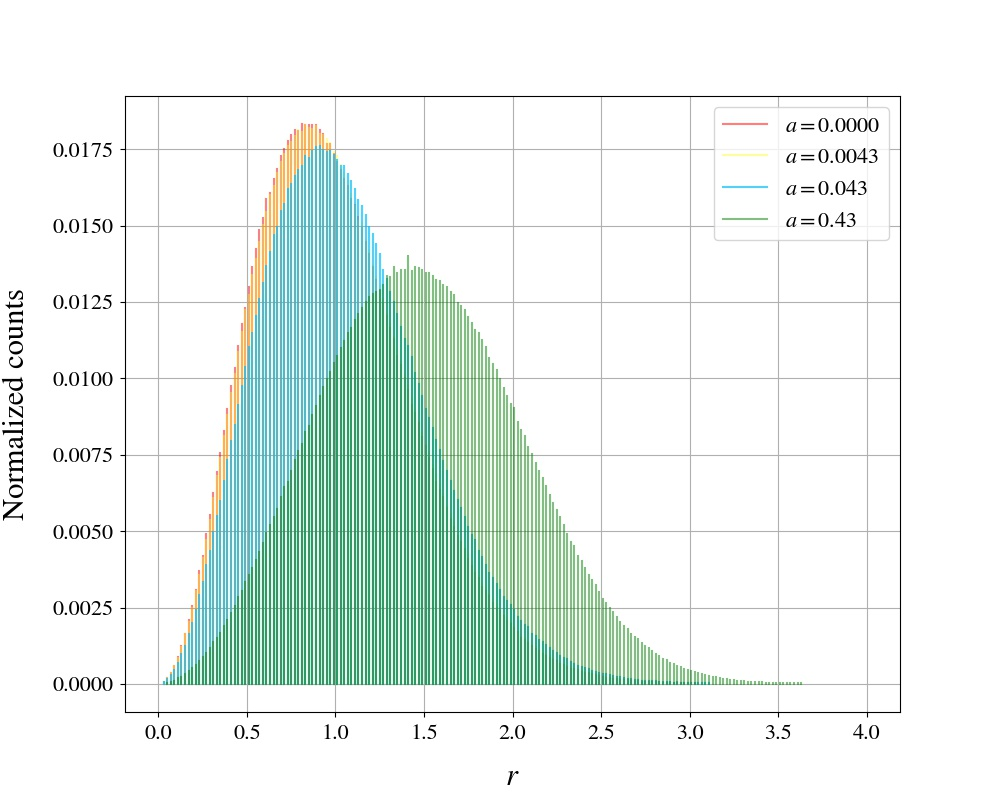
\includegraphics[scale=0.37]{images/onebody_density.jpg}
    \caption{One-body density as a function of the radial distance from the center of the chosen reference frame for a $3D$ system with $N=10$ particles described by an asymmetric gaussian wavefunction and inserted in a elliptical potential. The histograms are built for different values of $a$ in order to increase the effects introduced by the Jastrow factor in the wavefunction. The simulations were carried our exploiting the importance sampling with $N_{therm}=10^5$, $N_{steps}=2^{23}$, $\delta t =0.1$ and the $\alpha$ value deriving from the minimization of the energy (reported in Table \ref{tab:final_GS_energy}). Notice that the curves for $a=0$ and $a=0.0043$ are almost perfectly overlapped. }
    \label{fig:one_body_density_histogram}
\end{figure}


\begin{figure}[h!]
    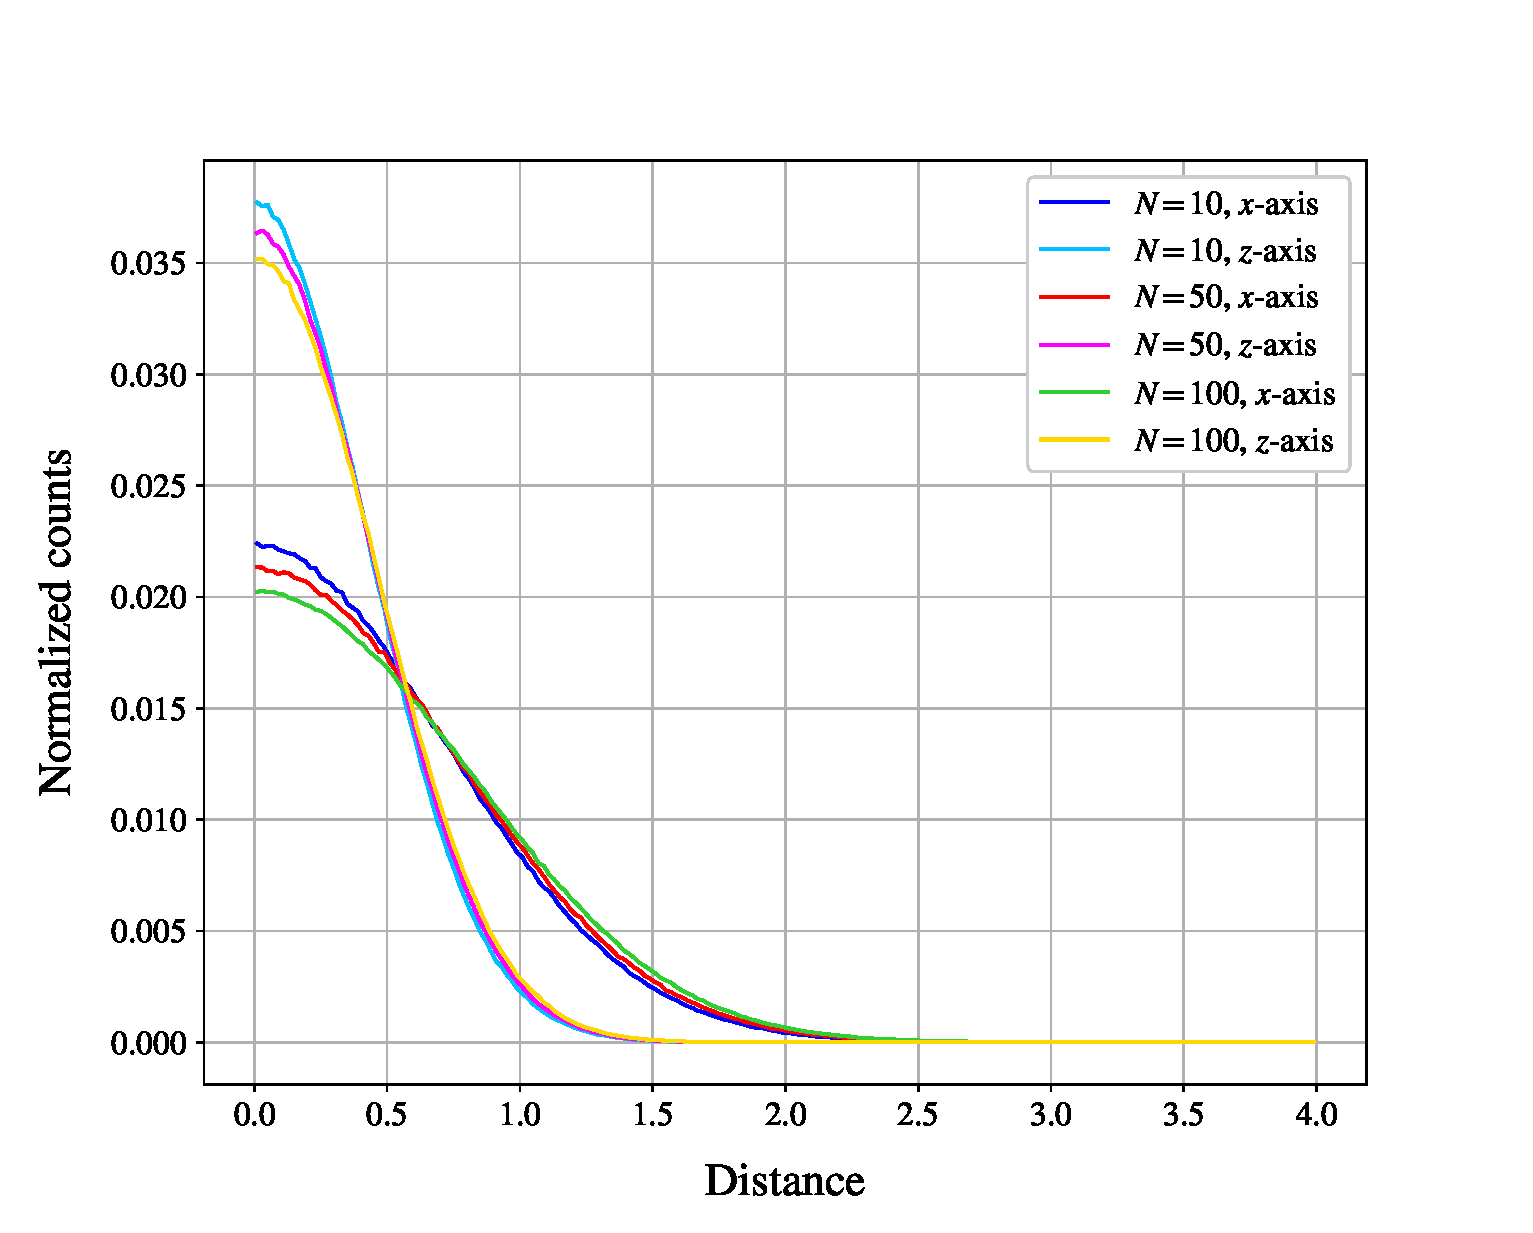
\includegraphics[scale=0.37]{images/spatial_distribution_x_z.eps}
    \caption{Particles' spatial distribution along the coordinates $x$ and $z$ for a system populated respectively by 10, 50 and 100 particles described by an asymmetric gaussian wavefunction and inserted in a elliptical potential. The simulations were carried our exploiting the importance sampling with $N_{therm}=10^5$, $N_{steps}=2^{23}$ steps and $\delta t =0.1$, setting $\alpha$ to the values reported in Table \ref{tab:final_GS_energy}. }
    \label{fig:spatial_distribution_x_z}
\end{figure}}

\newpage
\section*{APPENDIX}
\appendix
\section{LOCAL ENERGY: ANALYTICAL FORM}
\label{appendix:local_energy}
This section is devoted to show the detailed analytical derivation of the local energy formula in the general case. All the specific cases can be gotten from the final result reported below by setting properly the parameters of the system. For the sake of notation, we remind that we set $m=\hbar=\omega_{ho}=1$ and we introduce the variable $\bm{r}$ as a cumulative variable for $\{\bm{R}, \alpha, \beta\}$. The trial wavefunction describing the most general configuration for the system is reported in Eq.\,\ref{wavefunctions}, however to better face the analytical derivation we rewrite it here as:
\begin{equation*}
    \Psi_T(\mathbf{r} )=\left[ \prod_i^N g(\alpha,\beta,\mathbf{r}_i) \right] \exp{\left(\sum_{j<m}u(r_{jm})\right)}
\end{equation*} 
with 
\begin{equation}
    u(r_{ik})=\ln (f_{ik}) = \ln \left( 1-\frac{a}{r_{ik}} \right)
    \label{app:u_interaction}
\end{equation}
and
\begin{equation}
    g(\alpha,\beta,\mathbf{r}_i) = \exp{\left[-\alpha(x_i^2+y_i^2+\beta
    z_i^2)\right]}= \phi(\mathbf{r}_i)
    \label{app:gaussian}
\end{equation} 
The Hamiltonian of the system acquires the following form: 
\begin{equation*}
    \hat{H} = \frac{1}{2} \sum_i^N \left( - \nabla_{i}^2 + x_i^2 + y_i^2 +  \omega_{z}^2 z_i^2 \right) 
    +\sum_{i<j}^{N} V_{int}({\mathbf{r}}_i,{\mathbf{r}}_j)
\end{equation*}
We consider the %non trivial 
case of $r_{ij}>a,\, \forall i,j$, then  $V_{int}(\mathbf{r}_i,\mathbf{r}_j) = 0$. According to the definition of the local energy, we get
\begin{align}
    E_L(\mathbf{r}) &= \frac{1}{\Psi_T(\mathbf{r})} \hat{H} \Psi_T(\mathbf{r}) \nonumber\\
    &= -\frac{1}{2} \sum_k^N  \frac{\nabla_{k}^2\Psi_T(\mathbf{r})}{{\Psi_T(\mathbf{r})}} +\sum_k^N \frac{1}{2} \left(x_k^2 + y_k^2 + \omega_{z}^2 z_k^2 \right) 
    \label{app:localenergy_appendix}
\end{align}
One of the most nasty part of the derivation of the local energy is the evaluation of the kinetic term, which starts from the derivative of the trial wavefunction with respect to the position of the $k$-th particle: 
\begin{align}
    &\nabla_k\Psi_T(\mathbf{r}) = \nabla_k \bigg\{ \left[ \prod_i \phi(\mathbf{r}_i) \right] \exp{\left(\sum_{j<m}u(r_{jm})\right)} \bigg\} \nonumber\\
    &= \left[ \nabla_k \phi(\mathbf{r}_k) \right] \left[ \prod_{i \neq k} \phi(\mathbf{r}_i) \right] \exp{\left(\sum_{j<m}u(r_{jm})\right)} + \nonumber \\ 
    & + \left[\prod_i \phi(\mathbf{r}_i)  \right] \exp{\left(\sum_{j<m} u(r_{jm}) \right)} \nabla_k \left[ \sum_{j<m} u(r_{jm}) \right] \nonumber \\
    &= \left[ \nabla_k \phi(\mathbf{r}_k) \right] \left[ \prod_{i \neq k} \phi(\mathbf{r}_i) \right] \exp{\left(\sum_{j<m}u(r_{jm})\right)} + \nonumber\\
    & + \left[\prod_i \phi(\mathbf{r}_i) \right] \exp{\left(\sum_{j<m} u(r_{jm}) \right)} \left[ \sum_{j\neq k} \nabla_k u(r_{jk}) \right]
    \label{app:first_der_general}
\end{align}
In our specific case this yields to: 
\begin{align}
    &\nabla_k\Psi_T(\mathbf{r}) =\left[ \nabla_k  e^{  -\alpha(x_k^2 + y_k^2 + \beta z_k^2)} \right] \left[ \prod_{i \neq k}  e^{\left[ -\alpha(x_i^2 + y_i^2 + \beta z_i^2) \right]} \right] \times \nonumber \\
    & \times\left[ \prod_{j<m} \left( 1 - \frac{a}{r_{jm}} \right) \right] +  \left[\prod_i e^{ -\alpha (x_i^2 + y_i^2 + \beta z_i^2)} \right] \times \nonumber \\
    &\times \left[\prod_{j<m} \left( 1 - \frac{a}{r_{jm}} \right) \right] \left[ \sum_{j\neq k} \nabla_k \ln \left( 1 - \frac{a}{r_{jk}} \right) \right] \nonumber \\
    &= -2\alpha (x_k, y_k, \beta z_k) \Psi_T(\mathbf{r}) +  \sum_{j\neq k} \frac{1}{\left( 1 - \frac{a}{r_{jk}} \right)} \frac{a \mathbf{r}_{kj}}{r_{jk}^{3}} \Psi_T(\mathbf{r}) \nonumber \\
    &= \Psi_T(\mathbf{r}) \left[ -2\alpha (x_k, y_k, \beta z_k) + \sum_{j\neq k} \frac{a}{\left( r_{jk} - a \right) r_{jk}^2} \mathbf{r}_{kj} \right] 
    \label{app:first_der_specific}
\end{align}
To evaluate the second derivative we restart from Eq.\,\ref{app:first_der_general}.
Proceeding we get:
\begin{align*}
    &\nabla_k^2 \Psi_T(\mathbf{r}) = \left[ \nabla_k^2 \phi(\mathbf{r}_k) \right] \left[ \prod_{i \neq k} \phi(\mathbf{r}_i) \right] \exp{\left(\sum_{j<m}u(r_{jm})\right)} \\ 
    &+ \left[ \nabla_k \phi(\mathbf{r}_k) \right]  \left[ \prod_{i \neq k} \phi(\mathbf{r}_i) \right] \exp{\left(\sum_{j<m}u(r_{jm})\right)}\times \\
    & \times \left[ \sum_{j\neq k} \nabla_k u(r_{jk}) \right] + \left[ \nabla_k \phi(\mathbf{r}_k) \right] \left[ \prod_{i \neq k} \phi(\mathbf{r}_i) \right] \times \\
    & \times \exp{\left(\sum_{j<m} u(r_{jm}) \right)} \left[ \sum_{j\neq k} \nabla_k u(r_{jk}) \right] + \\ 
    &+\left[\prod_i \phi(\mathbf{r}_i) \right] \exp{\left(\sum_{j<m} u(r_{jm}) \right)} \left[ \sum_{j\neq k} \nabla_k^2 u(r_{jk}) \right] 
\end{align*}
Then dividing by $\Psi_T(\mathbf{r})$ we get: 
\begin{align*}
    &\frac{ \nabla_k^2 \Psi_T(\mathbf{r})}{\Psi_T(\mathbf{r})} = \frac{\nabla_k^2 \phi(\mathbf{r}_k)}{\phi(\mathbf{r}_k)} + 2 \frac{\nabla_k \phi(\mathbf{r}_k)}{\phi(\mathbf{r}_k)} \left[ \sum_{j\neq k} \nabla_k u(r_{jk}) \right] + \\
    & +\left[ \sum_{j\neq k} \nabla_k u(r_{jk}) \right]^2 + \left[ \sum_{j\neq k} \nabla_k^2 u(r_{jk}) \right] \\
    &= \frac{\nabla_k^2 \phi(\mathbf{r}_k)}{\phi(\mathbf{r}_k)} + 2 \frac{\nabla_k \phi(\mathbf{r}_k)}{\phi(\mathbf{r}_k)} \left[ \sum_{j\neq k} \nabla_k u(r_{jk}) \right] \nonumber\\
    & + \left[ \sum_{j\neq k} \sum_{m \neq k} \nabla_k u(r_{jk}) \nabla_k u(r_{mk}) \right] + \left[ \sum_{j\neq k} \nabla_k^2 u(r_{jk}) \right] 
\end{align*}
At this point we rewrite the gradient in spherical coordinates
\begin{equation*}
    \nabla f = \frac{\partial f}{\partial r} \frac{\mathbf{r}}{r} + \frac{1}{r} \frac{\partial f}{\partial \theta} \hat{\theta} + \frac{1}{\sin \theta} \frac{\partial f}{\partial \phi} \hat{\phi}
\end{equation*}
This choice simplifies the calculations, since the dependence of $u$ is limited to the relative distance between two particles. Applying then the gradient to $u(r_{jk})$, we get
\begin{equation*}
    \nabla_k u(r_{jk}) = \nabla_k (\mathbf{r}_k - \mathbf{r}_j) \nabla_{kj} u(r_{kj}) = \frac{\mathbf{r}_{kj}}{r_{kj}} \frac{du(r_{kj})}{dr_{kj}}
\end{equation*}
With the same reasoning, one can get also the expression for the Laplacian of $u(r_{jk})$ starting from
\begin{align*}
    \nabla^2 f &= \frac{1}{r^2} \frac{\partial}{\partial r} \left( r^2 \frac{\partial f}{\partial r} \right) + \frac{1}{r^2 \sin\theta } \frac{\partial }{\partial\theta} \left( \sin \theta \frac{\partial f}{\partial \theta} \right) + \\ 
    &+\frac{1}{r^2 \sin^2 \theta} \frac{\partial^2 f}{\partial \phi^2}
\end{align*}
which in our case reduces to
\begin{align*}
    &\nabla_k^2 u(r_{jk}) = \frac{1}{r_{jk}^2} \frac{\partial}{\partial r_{jk}} \left( r_{jk}^2 \frac{\partial u}{\partial r_{jk}} \right) \\ &= \frac{1}{r_{jk}^2}  \left( 2 r_{jk} \frac{\partial u}{\partial r_{jk}} + r_{jk}^2 \frac{\partial^2 u}{\partial r_{jk}^2} \right) = \frac{2}{r_{jk}} \frac{\partial u}{\partial r_{jk}} + \frac{\partial^2 u}{\partial r_{jk}^2}
\end{align*}
Joining all the terms evaluated up to now, we derive the expression for the kinetic energy term appearing in the expression for $E_L(\bm{r})$, namely
\begin{align}
     &\frac{ \nabla_k^2 \Psi_T(\mathbf{r})}{\Psi_T(\mathbf{r})} =  \underbrace{\frac{\nabla_k^2 \phi(\mathbf{r}_k)}{\phi(\mathbf{r}_k)}}_{\text{Term 1}} 
     + \underbrace{2 \frac{\nabla_k \phi(\mathbf{r}_k)}{\phi(\mathbf{r}_k)} \left[ \sum_{j\neq k}  \frac{\mathbf{r}_{kj}}{r_{kj}} \frac{du(r_{kj})}{dr_{kj}} \right]}_{\text{Term 2}} \nonumber\\
     & + \underbrace{\left[ \sum_{j\neq k} \sum_{m \neq k} \frac{\mathbf{r}_{kj}}{r_{kj}} \frac{du(r_{kj})}{dr_{kj}} \frac{\mathbf{r}_{km}}{r_{km}} \frac{du(r_{km})}{dr_{km}} \right]}_{\text{Term 3}} + \nonumber\\
     & + \underbrace{\left[ \sum_{j\neq k} \frac{2}{r_{jk}} \frac{\partial u(r_{jk})}{\partial r_{jk}} + \frac{\partial^2 u(r_{jk})}{\partial r_{jk}^2} \right]}_{\text{Term 4}} \nonumber \\
     \label{app:d2psi_psi_general}
\end{align}
Substituting the Eq.s\,\ref{app:u_interaction} and \ref{app:gaussian} into Eq.\,\ref{app:d2psi_psi_general} we can evaluate each term for the general case. 

\textbf{Term 1}
\begin{align*}
    \frac{\nabla_k^2 \phi(\mathbf{r}_k)}{\phi(\mathbf{r}_k)} = 2 \alpha \left[  2 \alpha (x_k^2 + y_k^2 + \beta^2 z_k^2 ) -2 -\beta \right]
\end{align*}

\textbf{Term 2}
\begin{align*}
    &2 \frac{\nabla_k \phi(\mathbf{r}_k)}{\phi(\mathbf{r}_k)} \left[ \sum_{j\neq k}  \frac{\mathbf{r}_{kj}}{r_{kj}} \frac{du(r_{kj})}{dr_{kj}} \right] = \\
    &=2 \left( -2 \alpha \left( x_k, y_k, \beta z_k \right) \right) \sum_{j\neq k}  \frac{\mathbf{r}_{kj}}{r_{kj}} \frac{a}{r_{kj} \left( r_{kj} - a \right)} \\
    &= -4 \alpha \left( x_k, y_k, \beta z_k \right) \cdot \sum_{j\neq k}  \frac{\mathbf{r}_{kj}}{r_{kj}} \frac{a}{r_{kj} \left( r_{kj} - a \right)} 
\end{align*}


\textbf{Term 3}
\begin{align*}
    &\sum_{j\neq k} \sum_{m \neq k} \frac{\mathbf{r}_{kj}}{r_{kj}} \frac{du(r_{kj})}{dr_{kj}} \frac{\mathbf{r}_{km}}{r_{km}} \frac{du(r_{km})}{dr_{km}} = \\
    &= \sum_{j\neq k} \sum_{m \neq k} \frac{\mathbf{r}_{kj}}{r_{kj}} \cdot  \frac{\mathbf{r}_{km}}{r_{km}} \frac{a}{r_{kj} \left( r_{kj} - a \right)} \frac{a}{r_{km} \left( r_{km} - a \right)} 
\end{align*}


\textbf{Term 4}
\begin{align*}
    &\sum_{j\neq k} \left[ \frac{2}{r_{jk}} \frac{\partial u(r_{jk})}{\partial r_{jk}} + \frac{\partial^2 u(r_{jk})}{\partial r_{jk}^2} \right] = \\
    &= \sum_{j\neq k} \left[ \frac{2}{r_{jk}} \frac{a}{r_{kj} \left( r_{kj} - a \right)} + \frac{a \left(a - 2 r_{kj} \right) }{r_{kj}^2 \left( r_{kj} - a \right)^2 } \right]
\end{align*}
Now, we have all the tools to evaluate analytically the local energy in Eq.\,\ref{app:localenergy_appendix}:

\begin{align*}
    &E_L(\mathbf{r})
    =-\frac{1}{2} \sum_i^N  \bigg\{ 2 \alpha \left[  2 \alpha (x_i^2 + y_i^2 + \beta^2 z_i^2 ) -2 -\beta \right] \\
    &\quad + \sum_{j\neq i} \frac{a}{r_{ij}^2 (r_{ij} - a)} \bigg\{ -4 \alpha \left( x_i, y_i, \beta z_i \right) \cdot \mathbf{r}_{ij} + 2 + \\ 
    & \quad \quad \quad + \frac{a - 2r_{ij}}{ r_{ij} - a } + \mathbf{r}_{ij} \cdot \sum_{m \neq i}   \frac{\mathbf{r}_{im}}{r_{im}} \frac{a}{r_{im} \left( r_{km} - a \right)} \bigg\} \bigg\} + \\
    & \quad\quad\quad\quad+ \frac{1}{2} 
    \sum_i^N (x_i^2 + y_i^2 + \omega_{z}^2 z_i^2) \\
    &= \alpha (2 + \beta) N -  2 \alpha^2 \sum_i^N (x_i^2 + y_i^2 + \beta^2 z_i^2 ) - \\
    &\quad \quad -\frac{1}{2} \sum_i^N \sum_{j\neq i} \frac{a}{r_{ij}^2 (r_{ij} - a)} \bigg\{ -4 \alpha \left( x_i, y_i, \beta z_i \right) \cdot \mathbf{r}_{ij} + 2 \\
    &\quad \quad \quad +\frac{a - 2r_{ij}}{ r_{ij} - a } + \mathbf{r}_{ij} \cdot \sum_{m \neq i}   \frac{\mathbf{r}_{im}}{r_{im}^2} \frac{a}{ \left( r_{km} - a \right)} \bigg\} \bigg\} \\
    &\quad \quad \quad \quad
    +\frac{1}{2} \sum_i^N (x_i^2 + y_i^2 + \omega_{z}^2 z_i^2) \\
    &= \alpha (2 + \beta) N + \sum_i^N \bigg[ (x_i^2 + y_i^2)\left(\frac{1}{2}- 2\alpha^2 \right) + \\
    & \quad + z_i^2\left( \frac{1}{2} \omega_z^2 - 2\alpha^2\beta^2 \right) \bigg] -  \frac{1}{2} \sum_i^N \sum_{j\neq i} \frac{a}{r_{ij}^2 (r_{ij} - a)} \times \\
    & \quad\quad \times \bigg\{ -4 \alpha \left( x_i, y_i, \beta z_i \right) \cdot \mathbf{r}_{ij} + 2 + \frac{a - 2r_{ij}}{r_{ij} - a } \\
    &\quad \quad \quad + \mathbf{r}_{ij} \cdot \sum_{m \neq i}   \frac{\mathbf{r}_{im}}{r_{im}^2} \frac{a}{\left( r_{km} - a \right)} \bigg\} \bigg\}
\end{align*}
which is the result reported in Eq.\,\ref{local_energy}. As previously stated, this is the most general result for the local energy in the context of this project, namely it corresponds to the the case of $N$ particles in an elliptical potential. However, by simply imposing conditions on $a$, $\beta$ and $\omega_z$ and possibly reducing the dimensionality of the system, every other treated case can be restored.

\section{GENERAL EXPRESSION FOR THE DRIFT FORCE}
\label{appendix:drift_force_general}
Appendix B
\section{GENERAL EXPRESSION FOR THE LOCAL ENERGY AS A FUNCTION OF ALPHA}
\label{appendix:local energy as function of alpha }
Here we aim to evaluate the derivative of the expected value of the local energy with respect to the variational parameter $\alpha$. This expression enters in the generation of a new value $\alpha_k$ in the context of the gradient descent method for the research of the minimum energy of a given system. Starting from the content of Eq.\,\ref{local_energy} and Eq.\,\ref{energy_integral}, we proceed as follows
\begin{align*}
    &\frac{\partial\langle E_L \rangle}{\partial\alpha} = \frac{\partial}{\partial \alpha} \left[ \int d\bm{R} P(\bm{R}, \bm{\alpha}) E_L(\bm{R}, \bm{\alpha}) \right]  \\
    &= \frac{\partial}{\partial \alpha} \left[ \frac{\int d\bm{R} \Psi_T^* \hat{H} \Psi_T}{\int d\bm{R} \Psi_T^* \Psi_T} \right]
\end{align*}
For the cases treated in the problem the trial wavefunction is real, leading to a simplification in the calculations. Furthermore, for the sake of reducing the notation, in the following steps we omit the dependences of $\Psi_T$, thus
\begin{align*}
\begin{split}
    &\frac{\partial\langle E_L \rangle}{\partial\alpha} = \frac{\partial}{\partial \alpha} \left[ \frac{\int d\bm{R} \Psi_T \hat{H} \Psi_T}{\int d\bm{R} \Psi_T^2} \right] \\
    &=\frac{1}{ \left[\int d\bm{R} \Psi_T^2 \right]^2} \bigg\{ \bigg[ \int d\bm{R} \overline{\Psi}_T \hat{H} \Psi_T + \int d\bm{R} \Psi_T \hat{H}\overline{\Psi}_T \bigg] \times \\
    &\times \left[\int d\bm{R} \Psi_T^2 \right] - \left[ \int d\bm{R} \Psi_T \hat{H} \Psi_T \right] \left[ \int d\bm{R} 2 \Psi_T \overline{\Psi}_T \right] \bigg\}
    \end{split}
\end{align*}
where $\overline{\Psi}_T$ is the derivative of $\Psi_T$ with respect to alpha. Using now the Hermiticity of $\hat{H}$, we get
\begin{equation*}
    \int d\bm{R} \Psi_T \hat{H} \overline{\Psi}_T = \langle \Psi_T \vert \hat{H} \vert \overline{\Psi}_T \rangle = \langle \hat{H} \Psi_T \vert \overline{\Psi}_T \rangle = \int d\bm{R} \overline{\Psi}_T \hat{H} \Psi_T
\end{equation*}
Thus we reduce to
\begin{align*}
    &\frac{\partial\langle E_L(\alpha) \rangle}{\partial\alpha} = \frac{2}{ \left[\int d\bm{R} \Psi_T^2 \right]^{\cancel{2}} } \left[ \int d\bm{R} \frac{\overline{\Psi}_T}{\Psi_T} \frac{\hat{H} \Psi_T}{\Psi_T} \Psi_T^2 \right] \cancel{\int d\bm{R} \Psi_T^2} - \\
    &- \frac{2}{ \left[\int d\bm{R} \Psi_T^2 \right]^2} \left[ \int d\bm{R} \frac{\hat{H} \Psi_T}{\Psi_T} \Psi_T^2 \right] \left[ \int d\bm{R}  \frac{\overline{\Psi}_T}{\Psi_T} \Psi_T^2 \right] \\
    &= 2\left[ \bigg\langle \frac{\overline{\Psi}_T}{\Psi_T} E_L \bigg\rangle - \bigg\langle \frac{\overline{\Psi}_T}{\Psi_T} \bigg\rangle \langle E_L \rangle \right]
\end{align*}
which is the result reported in Eq.\,\ref{dEnergy_dalpha}.

\bigskip

\end{multicols*}

\newpage
\begin{multicols}{2}
\printbibliography
\end{multicols}

\end{document}